\chapter{Eksperymenty}

\section{Środowisko obliczeniowe}

Badania eksperymentalne przeprowadzono na komputerze wyposażonym w procesor Intel Core i5-14600KF (12 rdzeni, taktowanie 3,49 GHz) oraz 16 GB pamięci RAM. Jako system operacyjny wykorzystano Ubuntu 24.04 LTS uruchomiony w środowisku WSL2. Wszystkie algorytmy zaimplementowano w języku Python 3.13 z użyciem bibliotek NumPy do operacji numerycznych, NetworkX do pracy z grafami oraz PuLP jako interfejs do solverów programowania liniowego. Podczas pomiarów wydajności mierzono wyłącznie czas wykonania algorytmów, pomijając operacje wejścia-wyjścia i przygotowania struktur danych.

\section{Metodologia eksperymentów}

\subsection{Protokół badawczy}

W celu zapewnienia kontrolowanych warunków eksperymentalnych, każdy algorytm uruchamiano w oddzielnym procesie systemowym z ustalonym limitem czasu wykonania wynoszącym 60 sekund. Przekroczenie tego limitu skutkowało oznaczeniem wyniku jako \texttt{timeout} i wykluczeniem go z analizy. Aby poprawić jakość rozwiązań początkowych, wszystkie algorytmy metaheurystyczne wykorzystywały technikę warm start, inicjalizując się rozwiązaniem uzyskanym przez algorytm zachłanny. Schemat powtórzeń eksperymentalnych przedstawiał się następująco:

\begin{itemize}
\item \textbf{Grafy syntetyczne}: 3 próbki na rozmiar, 2 powtórzenia na próbkę
\item \textbf{Grafy rzeczywiste}: 2 powtórzenia na graf ego
\end{itemize}

W procesie analizy uwzględniano jedynie te obserwacje, które zostały oznaczone flagą \texttt{valid=True} oraz nie nosiły statusu \texttt{timeout} ani \texttt{error}. Tak przygotowane dane poddano agregacji statystycznej z wykorzystaniem średniej arytmetycznej wraz z obliczeniem odchylenia standardowego.

\subsection{Analiza statystycznej istotności wyników}

Aby ocenić, czy zaobserwowane różnice w wydajności algorytmów mają charakter systematyczny czy przypadkowy, przeprowadzono szczegółową analizę statystyczną. Obliczono odchylenia standardowe oraz 95-procentowe przedziały ufności dla średnich wartości kosztów i czasów wykonania. Dodatkowo zastosowano nieparametryczne testy statystyczne do porównania wydajności poszczególnych metod.

\paragraph{Odchylenia standardowe i przedziały ufności}

Dla zbioru syntetycznego każda metoda miała co najmniej 100 obserwacji, co pozwoliło wyznaczyć wiarygodne 95-procentowe przedziały ufności:

\begin{itemize}
\item \textbf{ILPSolver}: średni koszt 1033 ± 269 (std ≈ 1371), czas 2492 ms ± 851 ms
\item \textbf{AntColonyOptimization}: średni koszt 1169 ± 149 (std ≈ 1115), czas 5124 ms ± 1232 ms
\item \textbf{TabuSearch}: średni koszt 1648 ± 259, czas 3298 ms ± 683 ms
\item \textbf{DominatingSetAlgorithm}: średni koszt 1678 ± 251, czas 16,7 ms ± 5,1 ms
\item \textbf{GreedyAlgorithm}: średni koszt 1706 ± 256, czas 0,96 ms ± 0,19 ms
\end{itemize}

Analiza przedziałów ufności wykazuje brak ich nakładania się między ILPSolverem a pozostałymi algorytmami, co stanowi silny dowód na systematyczną przewagę jakościową tej metody. Podobnie, różnice w wydajności między poszczególnymi metaheurystykami przewyższają szerokość ich przedziałów ufności, co świadczy o istotności statystycznej zaobserwowanych różnic.

Dla grafów ego z serwisu Facebook zastosowano mniejszą liczbę powtórzeń (12--20), co rezultuje szerszymi przedziałami ufności. Na przykład algorytm AntColonyOptimization osiągnął średni koszt 1155 ± 432 przy czasie wykonania 14~055 ms ± 8685 ms, podczas gdy TabuSearch uzyskał średni koszt 1463 ± 679 przy czasie 17~777 ms ± 10~432 ms. Należy zauważyć, że ILPSolver został uruchomiony jedynie dwukrotnie, w związku z czym jego zerowe odchylenie standardowe i przedział ufności dla kosztu nie mogą być interpretowane jako wskaźniki stabilności algorytmu.

\paragraph{Weryfikacja hipotez statystycznych}

Dla zbioru grafów syntetycznych zastosowano test Friedmana, analizując rangi kosztów i czasów wykonania z traktowaniem każdej instancji grafu jako osobnego bloku eksperymentalnego. Uzyskane wyniki wykazują istotność statystyczną na poziomie $p < 0{,}001$, co pozwala odrzucić hipotezę zerową o braku różnic między algorytmami. Przeprowadzony następnie test post-hoc Nemenyiego ujawnił następujące zależności:

\begin{itemize}
\item \textbf{ILPSolver} różni się istotnie od wszystkich pozostałych metod
\item \textbf{AntColonyOptimization} różni się od wszystkich heurystyk i większości metaheurystyk, lecz mniej wyraźnie od TabuSearch
\item \textbf{GreedyAlgorithm} i \textbf{RandomizedAlgorithm} tworzą grupę najsłabszych wyników i różnią się istotnie od wszystkich pozostałych
\end{itemize}

Ze względu na ograniczoną liczbę obserwacji dla grafów ego, zastosowane testy charakteryzują się mniejszą mocą statystyczną. Niemniej jednak wstępne wyniki sugerują zachowanie podobnej hierarchii wydajności algorytmów.

\subsection{Konfiguracja parametrów algorytmów}

W ramach prowadzonych eksperymentów zastosowano parametry domyślne biblioteki glopt dla wszystkich algorytmów metaheurystycznych. Świadomie zrezygnowano z przeprowadzenia specjalistycznego dostrajania parametrów, co stanowi uzasadniony kompromis między czasochłonnością badań a ich kompletnością:

\paragraph{AntColonyOptimization}
\begin{itemize}
\item Liczba mrówek: 20--30
\item Współczynnik parowania feromonu: 0.5
\item $\alpha = 1.0$ (wpływ feromonów)
\item $\beta = 2.0$ (wpływ heurystyki)
\item $q_0 = 0.9$ (prawdopodobieństwo wyboru najlepszego)
\item Długość ścieżki równa liczbie węzłów
\end{itemize}

\paragraph{GeneticAlgorithm}
\begin{itemize}
\item Populacja: 50 osobników
\item Krzyżowanie: 80\%
\item Mutacja: 20\%
\item Liczba pokoleń: 100
\item Selekcja: turniej (k=3)
\end{itemize}

\paragraph{TabuSearch}
\begin{itemize}
\item Długość listy tabu: około 10 elementów
\item Liczba iteracji: 1,000
\item Liczba sąsiadów na iterację: 10
\end{itemize}

\paragraph{SimulatedAnnealing}
\begin{itemize}
\item Temperatura początkowa: 1.0
\item Współczynnik chłodzenia: 0.95
\item Liczba iteracji: 1,000
\item Maksymalna liczba iteracji bez poprawy: 2,000
\end{itemize}

\section{Ograniczenia badań}

\subsection{Ograniczenia metodologiczne}

Przeprowadzone eksperymenty charakteryzują się kilkoma istotnymi ograniczeniami metodologicznymi. Po pierwsze, badania obejmowały jedynie trzy klasy grafów syntetycznych oraz 10 rzeczywistych sieci ego, co stanowi reprezentatywną, lecz ograniczoną próbę możliwych struktur sieciowych. Pominięto inne istotne rodzaje grafów, takie jak struktury z hiper-krawędziami, grafy skierowane czy sieci wielowarstwowe, przez co uzyskane wyniki mogą nie być w pełni reprezentatywne dla grafów o zasadniczo odmiennej topologii.

Po drugie, algorytm ILPSolver testowano wyłącznie na grafach małej wielkości, co uniemożliwia ocenę jego efektywności na sieciach większych rozmiarów. Jednocześnie algorytmy metaheurystyczne dla instancji o wielkości $n > 1000$ mogą wymagać dodatkowego dostrojenia parametrów w celu osiągnięcia optymalnej wydajności. Dodatkowo zakres analizy ograniczono do dwóch głównych konfiguracji licencyjnych: \emph{duolingo\_super} oraz \emph{roman\_domination}, co nie wyczerpuje pełnego spektrum możliwych modeli cenowych.

\subsection{Ograniczenia techniczne i pomiarowe}

Istotne ograniczenia wynikają również z aspektów technicznych eksperymentów. Zarówno proces generowania grafów syntetycznych, jak i działanie algorytmów metaheurystycznych opiera się na sekwencjach pseudolosowych. Mimo zastosowania deterministycznych seedów, pewien poziom wariancji wyników pozostaje nieunikniony, co może wpływać na powtarzalność rezultatów.

Pomiary czasu wykonania obejmują overhead systemowy, który może różnić się między platformami sprzętowymi. Szczególnie dla algorytmów długotrwałych (AntColony, TabuSearch) naturalne fluktuacje czasowe mogą być statystycznie istotne, co należy uwzględnić przy interpretacji wyników porównawczych.

Wymienione ograniczenia wymagają ostrożnej interpretacji uzyskanych rezultatów. Przedstawione wyniki należy traktować jako wskazówki metodologiczne dotyczące wyboru algorytmu w analogicznych warunkach eksperymentalnych. Należy mieć na uwadze, że względna hierarchia wydajności algorytmów mogłaby ulec zmianie w przypadku zastosowania innych parametrów metaheurystyk lub wydłużenia limitów czasowych. Niemniej jednak obserwowana spójność wyników między różnymi typami struktur grafowych dostarcza solidnej podstawy dla formułowania praktycznych rekomendacji.

\section{Charakterystyka zbiorów danych}

Materiał badawczy składał się z dwóch niezależnych kolekcji danych eksperymentalnych:

\begin{itemize}
\item \textbf{Syntetyczne grafy} -- trójelementowy zestaw generatorów (\emph{random}, \emph{small\_world}, \emph{scale\_free}) tworzył sieci o liczbie węzłów od 20 do 200 (co 20) oraz większe rozmiary 300, 400, 600, 800, 1000. Dla każdej kombinacji typu grafu i rozmiaru generowano trzy próbki, a następnie dla każdej z nich uruchamiano osiem algorytmów (\textbf{ILPSolver}, \textbf{GreedyAlgorithm}, \textbf{RandomizedAlgorithm}, \textbf{DominatingSetAlgorithm}, \textbf{AntColonyOptimization}, \textbf{SimulatedAnnealing}, \textbf{TabuSearch}, \textbf{GeneticAlgorithm}) w dwóch powtórzeniach. Badano dwie główne konfiguracje licencji: \emph{duolingo\_super} i \emph{roman\_domination}. Pomiar obejmował koszt całkowity \texttt{total\_cost}, czas wykonania \texttt{time\_ms} oraz poprawność rozwiązania \texttt{valid}.

\item \textbf{Grafy facebook ego} -- dziesięć grafów ego pobranych z bazy SNAP (rozmiary 53--1035 węzłów) reprezentowało sieci rzeczywiste. Uruchomiono te same algorytmy i konfiguracje licencji, odnotowując te same metryki co dla grafów syntetycznych.
\end{itemize}

Dla obu kolekcji danych zastosowano jednolitą procedurę filtracji, wykluczając z analizy wyniki oznaczone statusami \texttt{timeout} lub \texttt{error}, a także obserwacje niespełniające warunków poprawności (\texttt{valid=False}).

\section{Analiza wyników dla grafów syntetycznych}

Po zastosowaniu procedur filtracji na zbiorze grafów syntetycznych uzyskano ponad 12 tysięcy prawidłowych uruchomień algorytmów, z których 1972 dotyczyło konfiguracji licencyjnej \emph{duolingo\_super}. W dalszej analizie skupiono się na wynikach uzyskanych dla tej konfiguracji jako najbardziej reprezentatywnej.

\subsection{Analiza rozkładów kosztów i czasów wykonania}

Rysunek \ref{fig:synthetic_cost_boxplot} przedstawia rozkład całkowitych kosztów \texttt{total\_cost} w przekroju badanych algorytmów. Wyniki wyraźnie wskazują na dominację \textbf{ILPSolvera}, który osiąga najniższe wartości kosztowe, aczkolwiek jego zastosowanie ogranicza się do grafów o niewielkich rozmiarach. W grupie algorytmów metaheurystycznych najlepszą jakość rozwiązań demonstruje \textbf{AntColonyOptimization}, podczas gdy \textbf{GreedyAlgorithm} charakteryzuje się znacznie wyższymi kosztami. Dla porównania, \textbf{RandomizedAlgorithm} służący jako baseline potwierdza skuteczność metod heurystycznych -- wszystkie badane algorytmy przewyższają losowe przydzielanie licencji.

\begin{figure}[H]
  \centering
  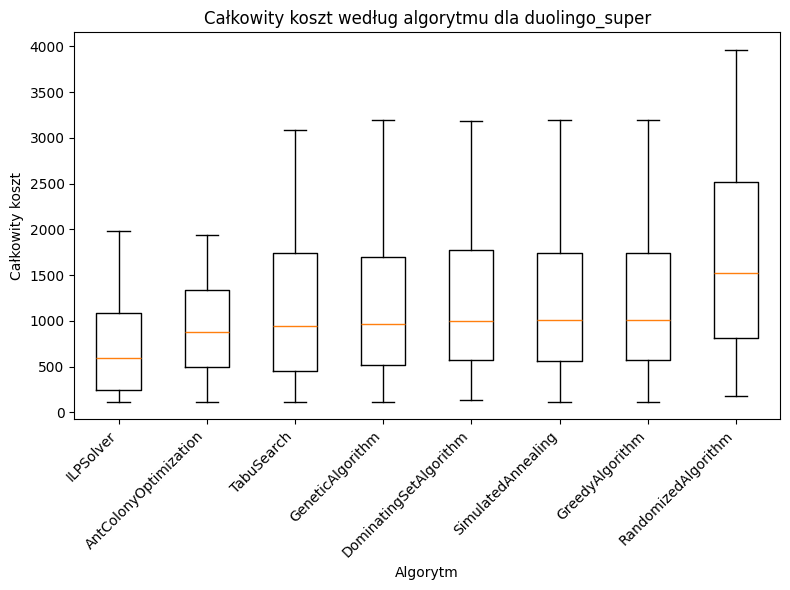
\includegraphics[width=0.7\linewidth]{assets/figures/synthetic_cost_boxplot.png}
  \caption{Całkowity koszt według algorytmu dla konfiguracji duolingo\_super (grafy syntetyczne).}
  \label{fig:synthetic_cost_boxplot}
\end{figure}

Analiza czasów wykonania, przedstawiona na rysunku \ref{fig:synthetic_time_boxplot} w skali logarytmicznej, ujawnia wyraźne zróżnicowanie wydajnościowe algorytmów. Metody Greedy oraz Randomized wykazują niekwestionowaną dominację pod względem szybkości działania, podczas gdy algorytmy metaheurystyczne i ILPSolver wymagają czasu wykonania mierzonego w sekundach lub dziesiątkach sekund.

\begin{figure}[H]
  \centering
  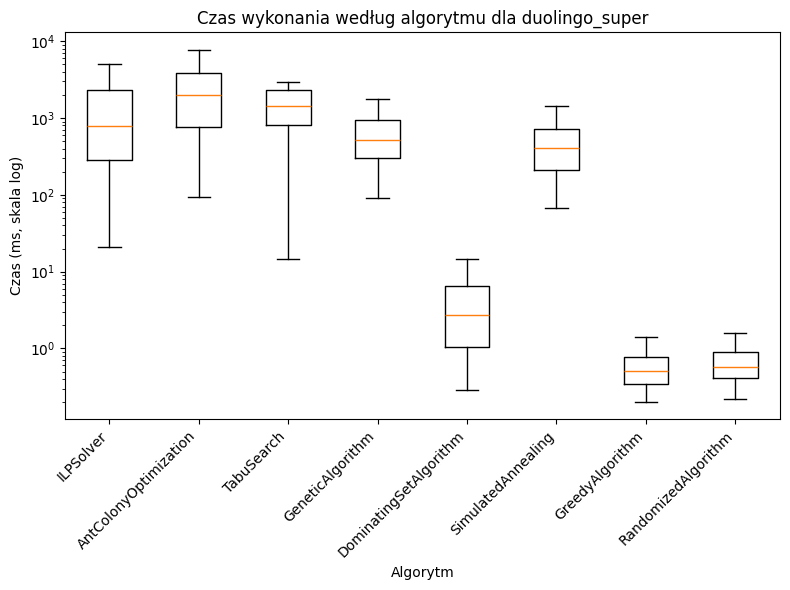
\includegraphics[width=0.7\linewidth]{assets/figures/synthetic_time_boxplot.png}
  \caption{Czas wykonania według algorytmu dla konfiguracji duolingo\_super (grafy syntetyczne).}
  \label{fig:synthetic_time_boxplot}
\end{figure}

\subsection{Zależność wydajności od wielkości grafu}

Analiza wpływu liczby węzłów na średni koszt rozwiązań, przedstawiona na rysunku \ref{fig:synthetic_cost_vs_nodes}, wykazuje tendencję wzrostową kosztów wraz ze zwiększaniem się rozmiaru grafu. \textbf{ILPSolver} utrzymuje pozycję lidera pod względem jakości rozwiązań dla grafów o wielkości do około $n \approx 200$ węzłów. \textbf{AntColonyOptimization} plasuje się na drugiej pozycji, jednak dla grafów większych rozmiarów obserwuje się stopniowy wzrost generowanych kosztów. Pozostałe algorytmy metaheurystyczne tworzą względnie zwartą grupę wyników, podczas gdy metody Greedy i Randomized charakteryzują się stałym, lecz wysokim poziomem kosztów niezależnie od rozmiaru grafu.

\begin{figure}[H]
  \centering
  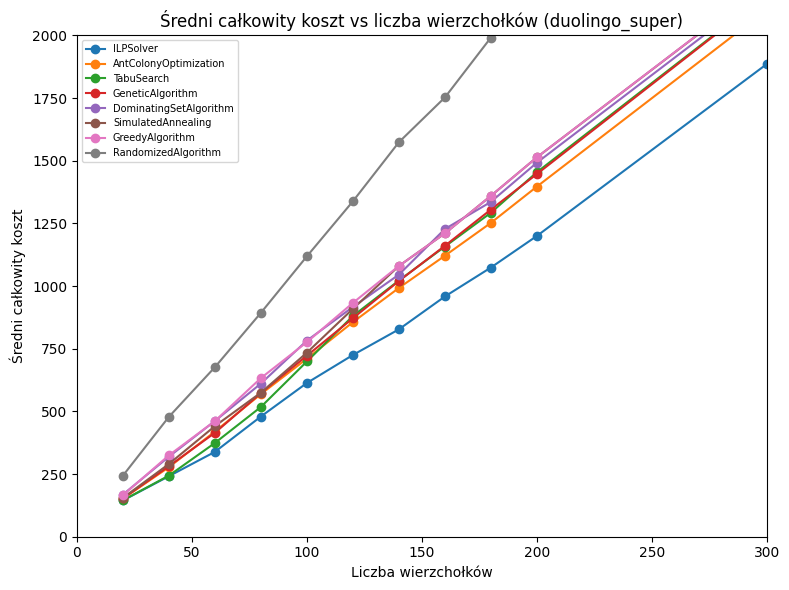
\includegraphics[width=0.7\linewidth]{assets/figures/synthetic_cost_vs_nodes.png}
  \caption{Średni całkowity koszt vs liczba węzłów (grafy syntetyczne).}
  \label{fig:synthetic_cost_vs_nodes}
\end{figure}

Analogicznie, czasy obliczeń pokazane na rysunku \ref{fig:synthetic_time_vs_nodes} w skali logarytmicznej rosną niemal liniowo z liczbą węzłów dla metaheurystyk. Greedy i Randomized są prawie niezależne od rozmiaru, a DominatingSetAlgorithm i SimulatedAnnealing plasują się pośrodku.

\begin{figure}[H]
  \centering
  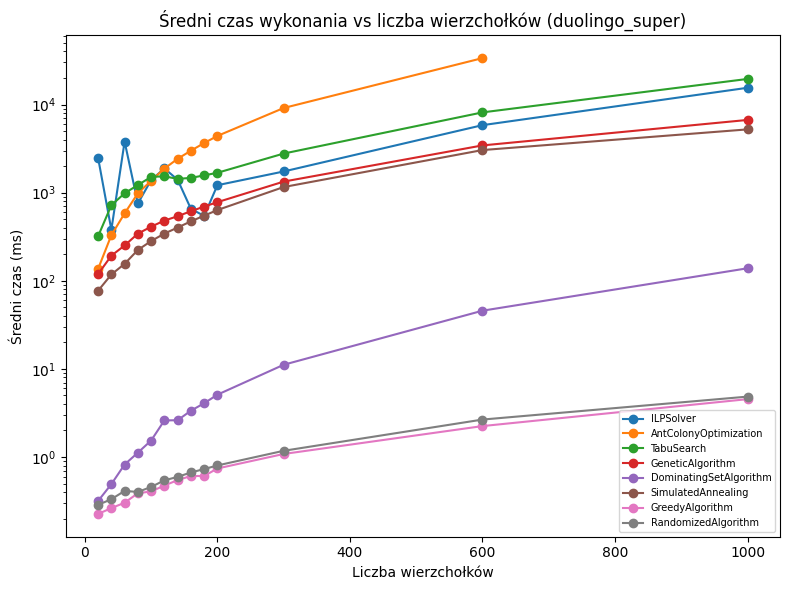
\includegraphics[width=0.7\linewidth]{assets/figures/synthetic_time_vs_nodes.png}
  \caption{Średni czas wykonania vs liczba węzłów (grafy syntetyczne).}
  \label{fig:synthetic_time_vs_nodes}
\end{figure}

\subsection{Kompromis koszt--czas}

Wykres Pareto (rys. \ref{fig:synthetic_pareto}) ilustruje zależność między kosztem a czasem. Najkorzystniejsze punkty należą do \textbf{ILPSolvera} i \textbf{AntColonyOptimization}, lecz czas drugiego z nich jest wielokrotnie większy. \textbf{TabuSearch} i \textbf{GeneticAlgorithm} zapewniają przyzwoite koszty przy umiarkowanych czasach, natomiast Greedy i Randomized pozostają najszybsze kosztem jakości.

\begin{figure}[H]
  \centering
  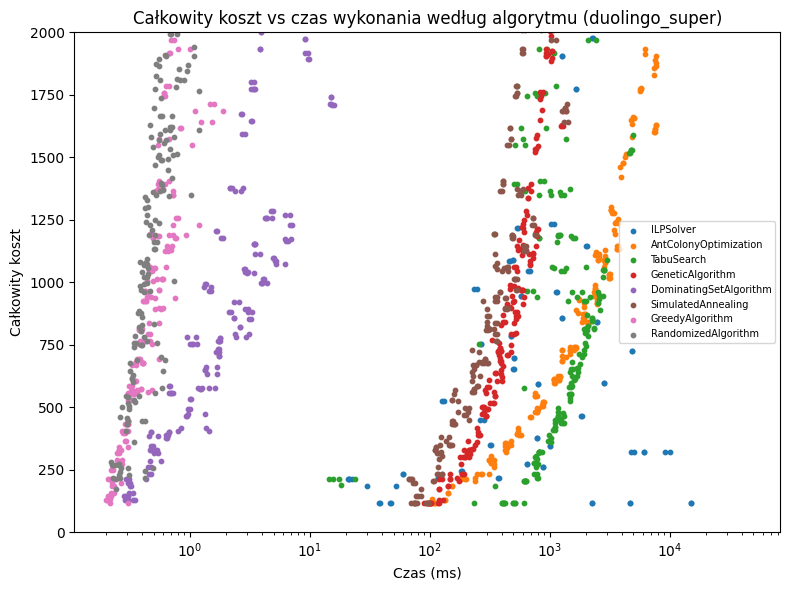
\includegraphics[width=0.7\linewidth]{assets/figures/synthetic_pareto.png}
  \caption{Całkowity koszt vs czas wykonania (grafy syntetyczne).}
  \label{fig:synthetic_pareto}
\end{figure}

\subsection{Koszt na węzeł i rozrzut czasów}

Rozkład kosztu w przeliczeniu na węzeł (rys. \ref{fig:synthetic_cost_per_node}) potwierdza przewagę ILPSolvera i AntColonyOptimization, a rozrzut czasów w zależności od liczby węzłów (rys. \ref{fig:synthetic_time_scatter}) pokazuje silną zależność czasową dla metaheurystyk (współczynnik korelacji z liczbą węzłów sięga 0,90) i niewielki wpływ gęstości grafu (korelacje ujemne --0,05 do --0,30).

\begin{figure}[H]
  \centering
  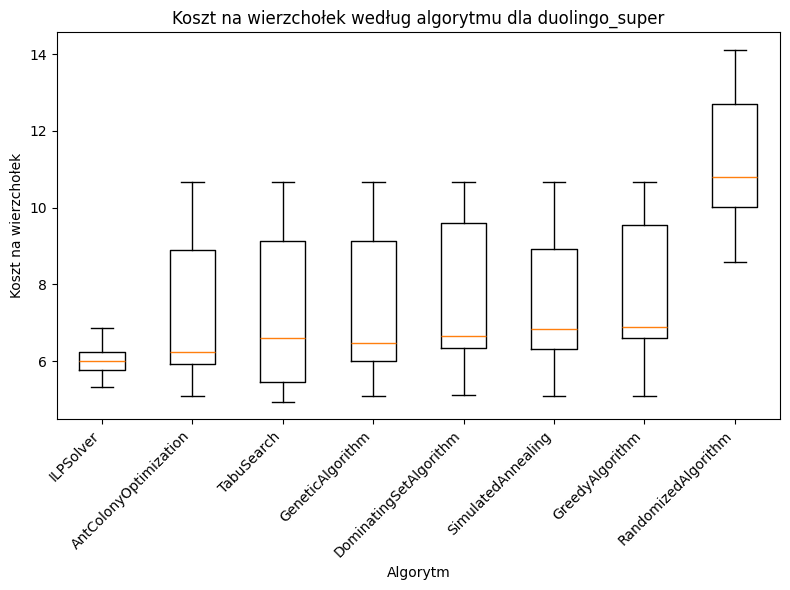
\includegraphics[width=0.7\linewidth]{assets/figures/synthetic_cost_per_node.png}
  \caption{Koszt na węzeł według algorytmu (grafy syntetyczne).}
  \label{fig:synthetic_cost_per_node}
\end{figure}

\begin{figure}[H]
  \centering
  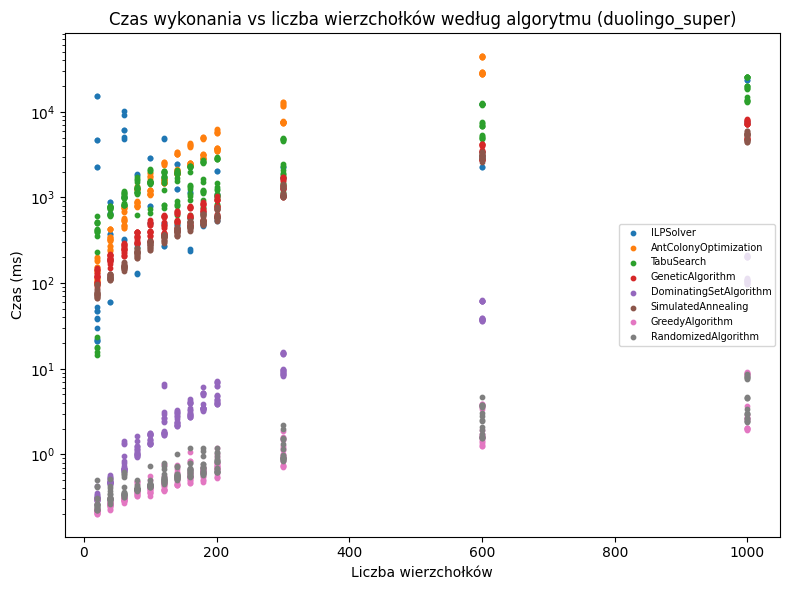
\includegraphics[width=0.7\linewidth]{assets/figures/synthetic_time_scatter.png}
  \caption{Czas wykonania vs liczba węzłów (grafy syntetyczne).}
  \label{fig:synthetic_time_scatter}
\end{figure}

\section{Analiza grafów facebook ego}

Eksperymenty na sieciach ego objęły 10 grafów o wielkości 53--1035 węzłów. Z 320 uruchomień zachowano 288 poprawnych obserwacji.

\subsection{Rozkład kosztów i czasów}

Rysunek \ref{fig:facebook_cost_boxplot} przedstawia koszty dla \emph{duolingo\_super} na grafach facebookowych. \textbf{ILPSolver} ponownie osiąga najniższe koszty, lecz wykonał się tylko dla dwóch najmniejszych grafów. \textbf{AntColonyOptimization} zapewnia kolejny najniższy koszt, ale jest bardzo wolny. Heurystyki Greedy i Randomized są najszybsze, lecz mają najwyższe koszty.

\begin{figure}[H]
  \centering
  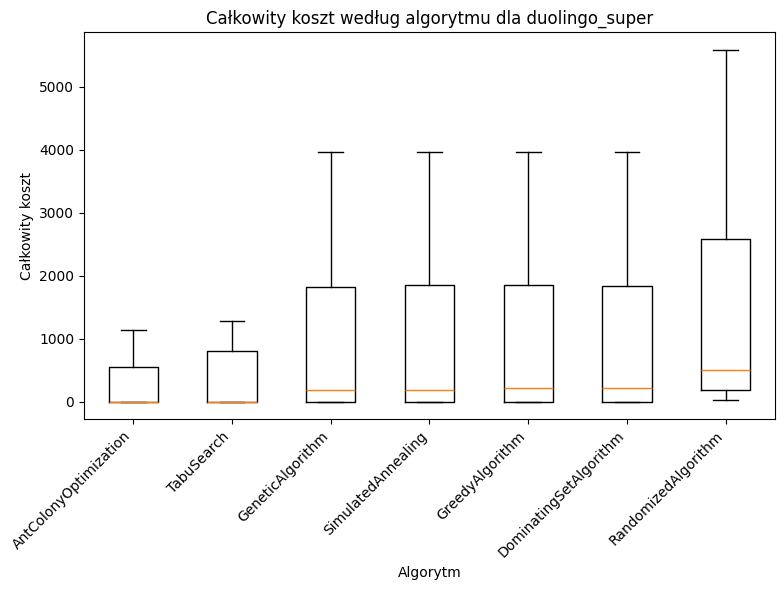
\includegraphics[width=0.7\linewidth]{assets/figures/facebook_cost_boxplot.png}
  \caption{Całkowity koszt według algorytmu dla konfiguracji duolingo\_super (grafy facebook).}
  \label{fig:facebook_cost_boxplot}
\end{figure}

Czas działania (rys. \ref{fig:facebook_time_boxplot}) pokazuje, że metaheurystyki na grafach ego są jeszcze wolniejsze niż na grafach syntetycznych -- czas \textbf{AntColonyOptimization} i \textbf{TabuSearch} sięga 8--10 s. ILPSolver rozwiązuje tylko małe instancje w $\sim$0,3 s.

\begin{figure}[H]
  \centering
  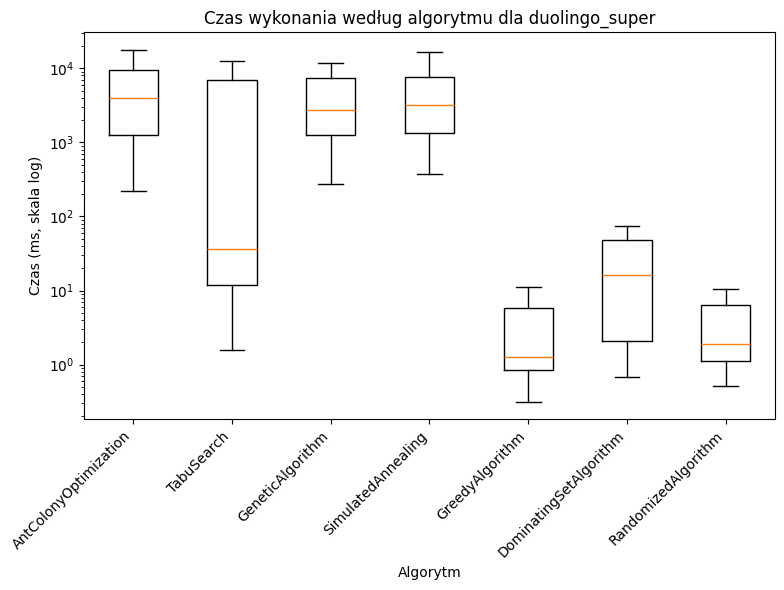
\includegraphics[width=0.7\linewidth]{assets/figures/facebook_time_boxplot.png}
  \caption{Czas wykonania według algorytmu dla konfiguracji duolingo\_super (grafy facebook).}
  \label{fig:facebook_time_boxplot}
\end{figure}

\subsection{Zależność od liczby węzłów}

Średnie koszty dla grafów ego (rys. \ref{fig:facebook_cost_vs_nodes}) rosną wraz z rozmiarem, lecz skala jest mniejsza -- ILPSolver ($n = 2$) i AntColony zapewniają koszty do $\sim$1500. Pozostałe algorytmy szybko rosną powyżej 2000, zwłaszcza GeneticAlgorithm i SimulatedAnnealing.

\begin{figure}[H]
  \centering
  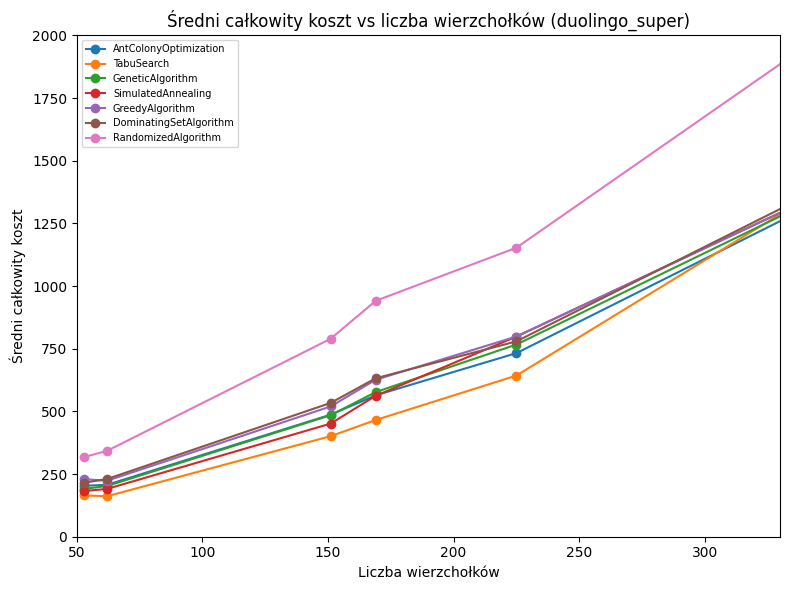
\includegraphics[width=0.7\linewidth]{assets/figures/facebook_cost_vs_nodes.png}
  \caption{Średni całkowity koszt vs liczba węzłów (grafy facebook).}
  \label{fig:facebook_cost_vs_nodes}
\end{figure}

Wykres czasów (rys. \ref{fig:facebook_time_vs_nodes}) ukazuje, że czasy \textbf{AntColonyOptimization} i \textbf{TabuSearch} zwiększają się mocno wraz z rozmiarem grafu, osiągając nawet 10 s. \textbf{GreedyAlgorithm} i \textbf{RandomizedAlgorithm} pozostają najkrótsze (ms) niezależnie od wielkości.

\begin{figure}[H]
  \centering
  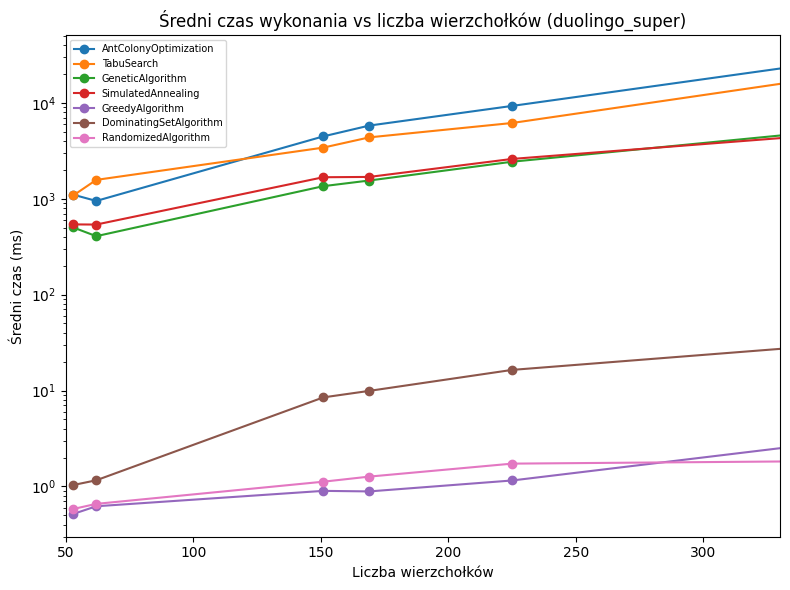
\includegraphics[width=0.7\linewidth]{assets/figures/facebook_time_vs_nodes.png}
  \caption{Średni czas wykonania vs liczba węzłów (grafy facebook).}
  \label{fig:facebook_time_vs_nodes}
\end{figure}

\subsection{Kompromis koszt--czas i koszt na węzeł}

Wykres Pareto (rys. \ref{fig:facebook_pareto}) dla grafów ego pokazuje mniejszą liczbę punktów: ILPSolver i AntColonyOptimization tworzą front optymalny; TabuSearch, GeneticAlgorithm i SimulatedAnnealing tworzą kompromisy; Greedy i Randomized są ultraszybkie, lecz pozostają w górnej części wykresu.

\begin{figure}[H]
  \centering
  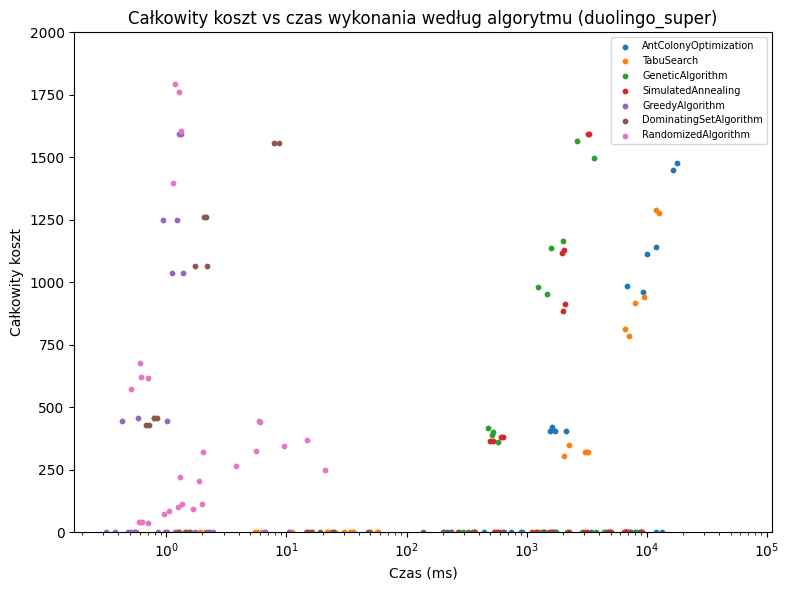
\includegraphics[width=0.7\linewidth]{assets/figures/facebook_pareto.png}
  \caption{Całkowity koszt vs czas wykonania (grafy facebook).}
  \label{fig:facebook_pareto}
\end{figure}

Rozkład kosztu na węzeł (rys. \ref{fig:facebook_cost_per_node}) potwierdza, że różnice między algorytmami są istotne, a realne grafy charakteryzują się niższym kosztem na węzeł niż syntetyczne.

\begin{figure}[H]
  \centering
  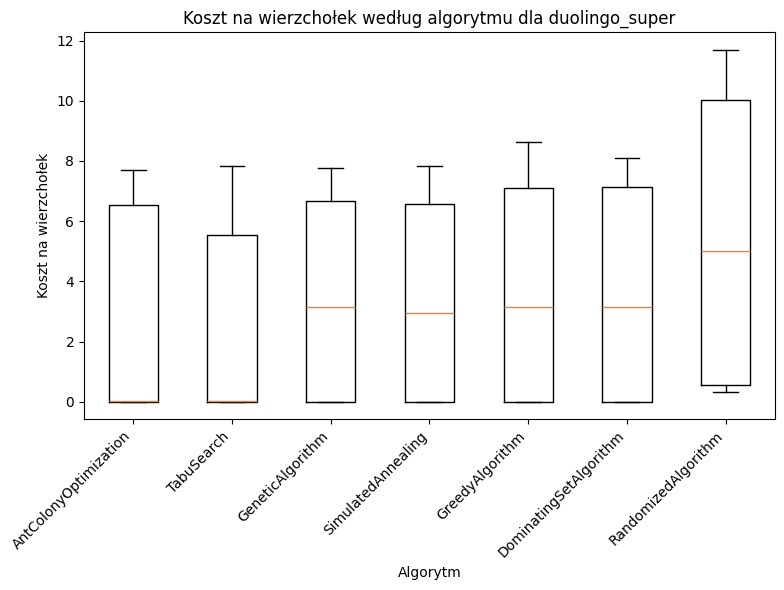
\includegraphics[width=0.7\linewidth]{assets/figures/facebook_cost_per_node.png}
  \caption{Koszt na węzeł według algorytmu (grafy facebook).}
  \label{fig:facebook_cost_per_node}
\end{figure}

Rozrzut czasów w zależności od liczby węzłów (rys. \ref{fig:facebook_time_scatter}) pokazuje, że metaheurystyki wykazują silniejszą zależność od rozmiaru grafu (korelacje $\sim$0,9) niż heurystyki.

\begin{figure}[H]
  \centering
  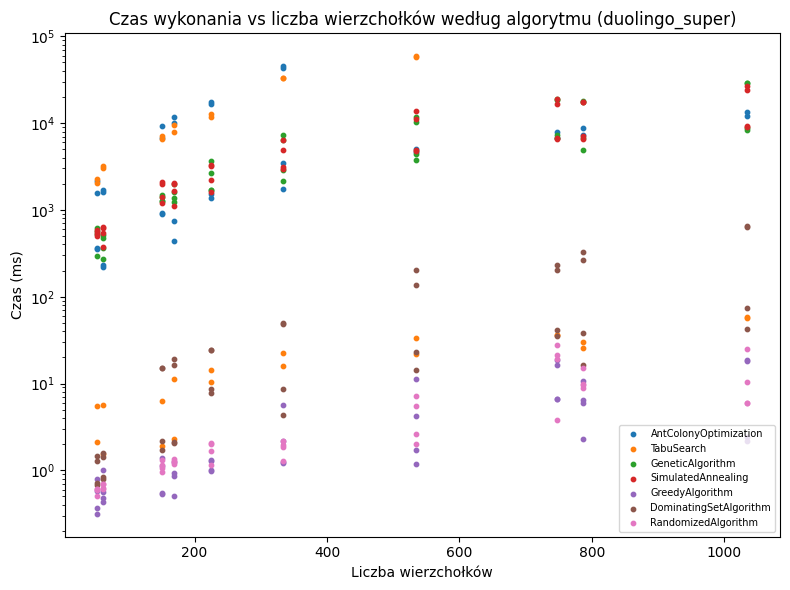
\includegraphics[width=0.7\linewidth]{assets/figures/facebook_time_scatter.png}
  \caption{Czas wykonania vs liczba węzłów (grafy facebook).}
  \label{fig:facebook_time_scatter}
\end{figure}

\section{Synteza wyników i wnioski}

Przeprowadzona analiza porównawcza grafów syntetycznych oraz rzeczywistych sieci ego z Facebooka ujawnia spójne wzorce wydajnościowe, aczkolwiek między tymi zbiorami danych obserwuje się różnice w rozkładach kosztów i czasów wykonania.

\begin{itemize}
\item \textbf{Jakość.} W obu zestawach \textbf{ILPSolver} osiąga najniższe koszty, lecz jest ograniczony do małych grafów. Z metaheurystyk najlepiej wypada \textbf{AntColonyOptimization} (niski koszt, długi czas), następnie \textbf{TabuSearch} i \textbf{GeneticAlgorithm}. \textbf{GreedyAlgorithm} generuje wysokie koszty, ale jest bardzo szybki. \textbf{RandomizedAlgorithm} służy jako baseline potwierdzający, że wszystkie pozostałe algorytmy znacznie przewyższają losowe przydzielanie.

\item \textbf{Czas.} \textbf{GreedyAlgorithm} charakteryzuje się bardzo krótkim czasem wykonania, podobnie jak baseline \textbf{RandomizedAlgorithm}; \textbf{DominatingSetAlgorithm} i \textbf{SimulatedAnnealing} oferują lekko lepsze wyniki przy nadal krótkim czasie. \textbf{AntColonyOptimization} i \textbf{TabuSearch} są wielokrotnie wolniejsze i stają się niepraktyczne dla grafów ego.

\item \textbf{Skalowalność.} Dla grafów syntetycznych czasy metaheurystyk rosną w przybliżeniu wykładniczo z liczbą węzłów; w grafach ego ten wzrost jest jeszcze większy. Koszty rosną prawie liniowo z rozmiarem w obu zbiorach.

\item \textbf{Realne vs syntetyczne.} Koszty w grafach ego są nieco niższe, ale czasy metaheurystyk dłuższe, co sugeruje, że realne sieci mają bardziej złożoną strukturę. Kolejność algorytmów pozostaje jednak taka sama.
\end{itemize}

Konkludując, strategia wyboru algorytmu powinna uwzględniać zarówno rozmiar analizowanej sieci, jak i akceptowalny kompromis między kosztem licencji a czasem potrzebnym na obliczenia. Dla sieci małych rozmiarów ILPSolver stanowi bezalternatywne rozwiązanie ze względu na optimalność uzyskiwanych wyników. W przypadku grafów średnich i dużych rozmiarów rekomenduje się zastosowanie algorytmów \textbf{TabuSearch} lub \textbf{GeneticAlgorithm}, które oferują satysfakcjonujący kompromis między czasem wykonania a jakością rozwiązań. Gdy priorytetem jest minimalizacja czasu obliczeń, alternatywą może być \textbf{GreedyAlgorithm}, choć przy akceptacji znacząco wyższych kosztów licencyjnych niż w przypadku metod metaheurystycznych.



\section{Wyniki eksperymentów}

\subsection{Wydajność algorytmów dla konfiguracji duolingo\_super}

Na wykresach poniżej przedstawiono zachowanie różnych algorytmów dla konfiguracji licencji duolingo\_super na grafach syntetycznych.

\begin{figure}[H]
  \centering
  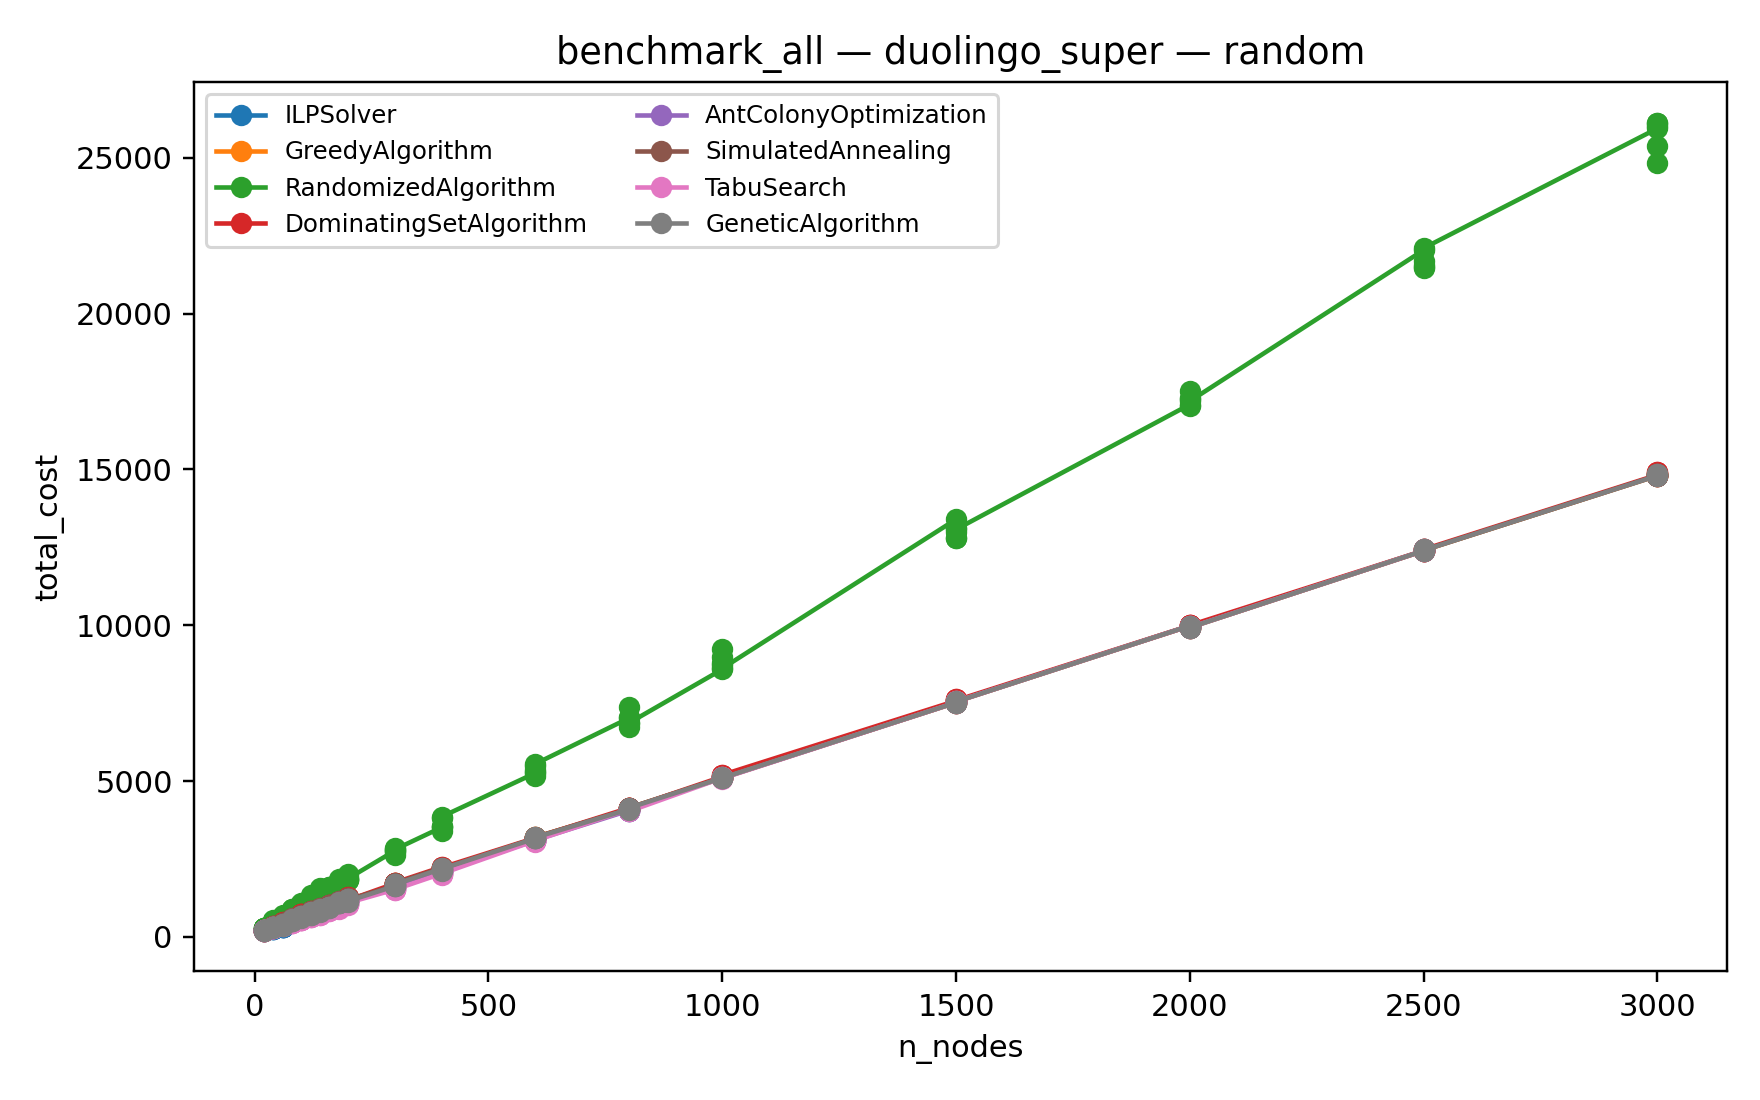
\includegraphics[width=0.48\linewidth]{assets/figures/ba_random_duo_cost_vs_n.png}
  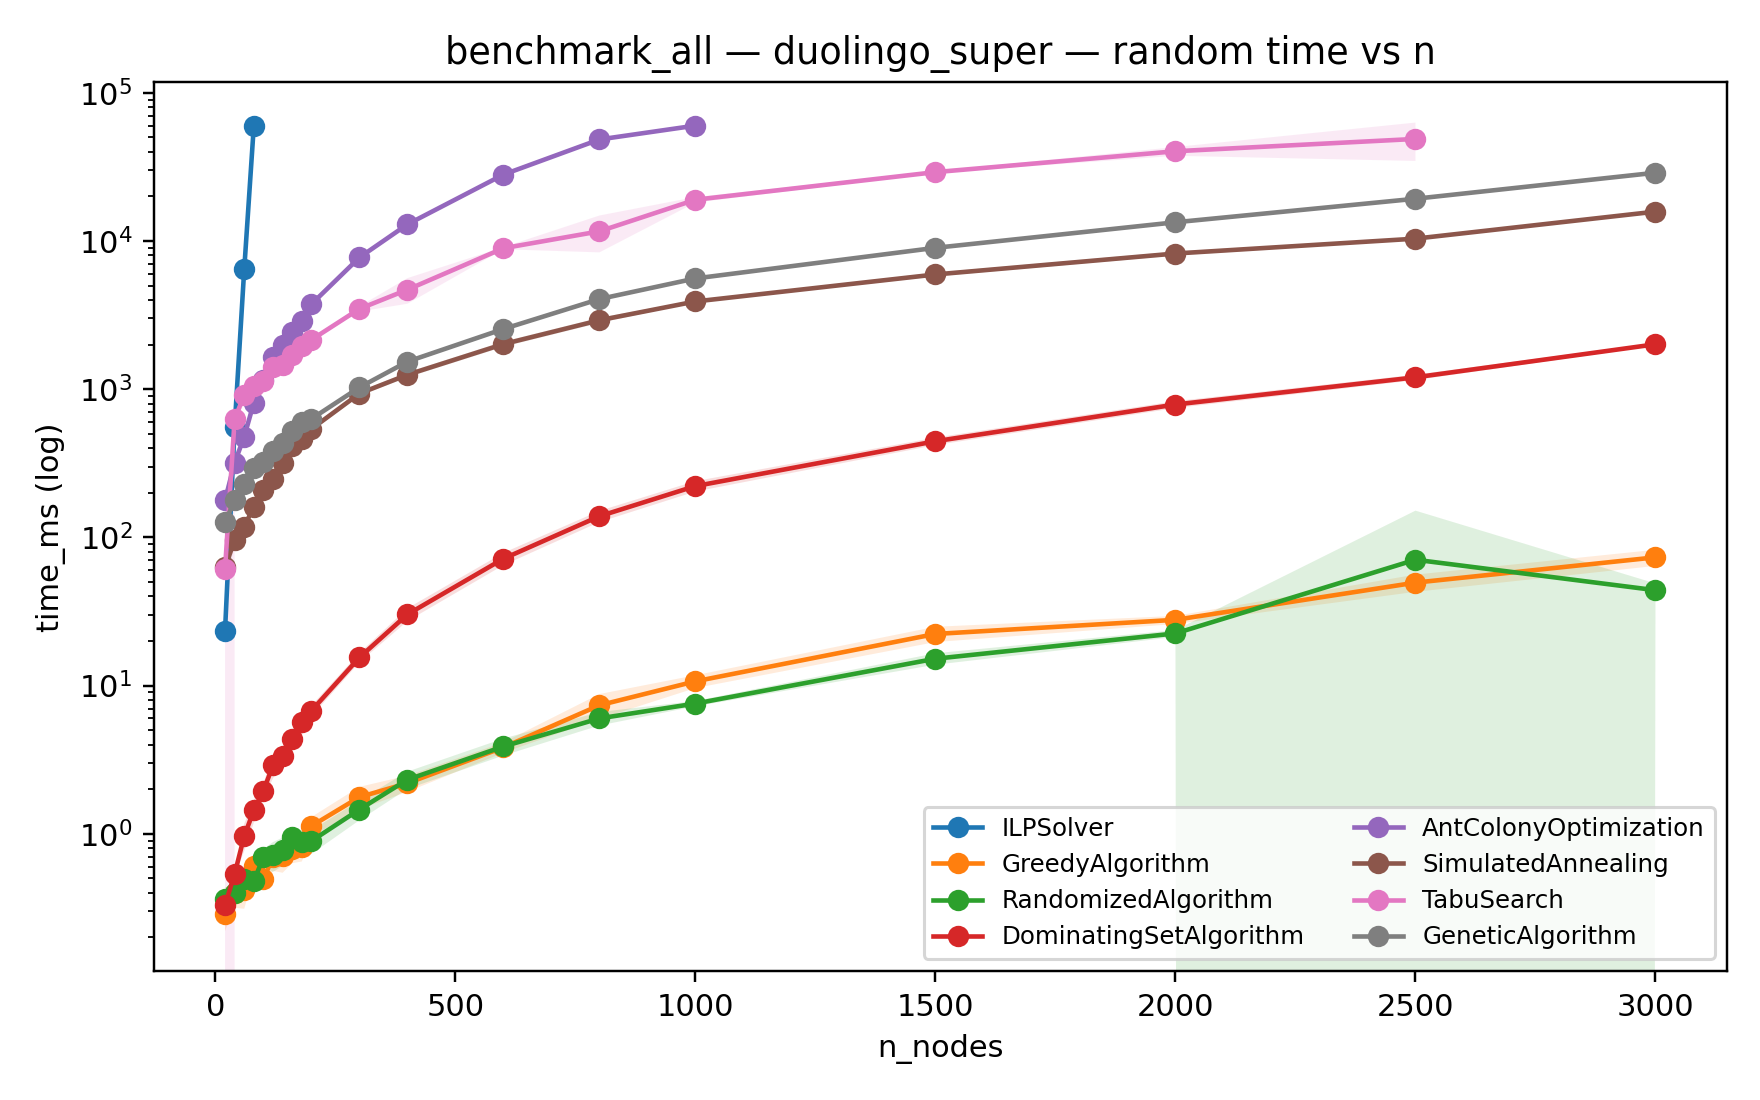
\includegraphics[width=0.48\linewidth]{assets/figures/ba_random_duo_time_vs_n.png}
  \caption{Grafy losowe (konf. duolingo\_super) -- koszt na wierzchołek i czas wykonania vs liczba wierzchołków.}
  \label{fig:random_performance}
\end{figure}

\begin{figure}[H]
  \centering
  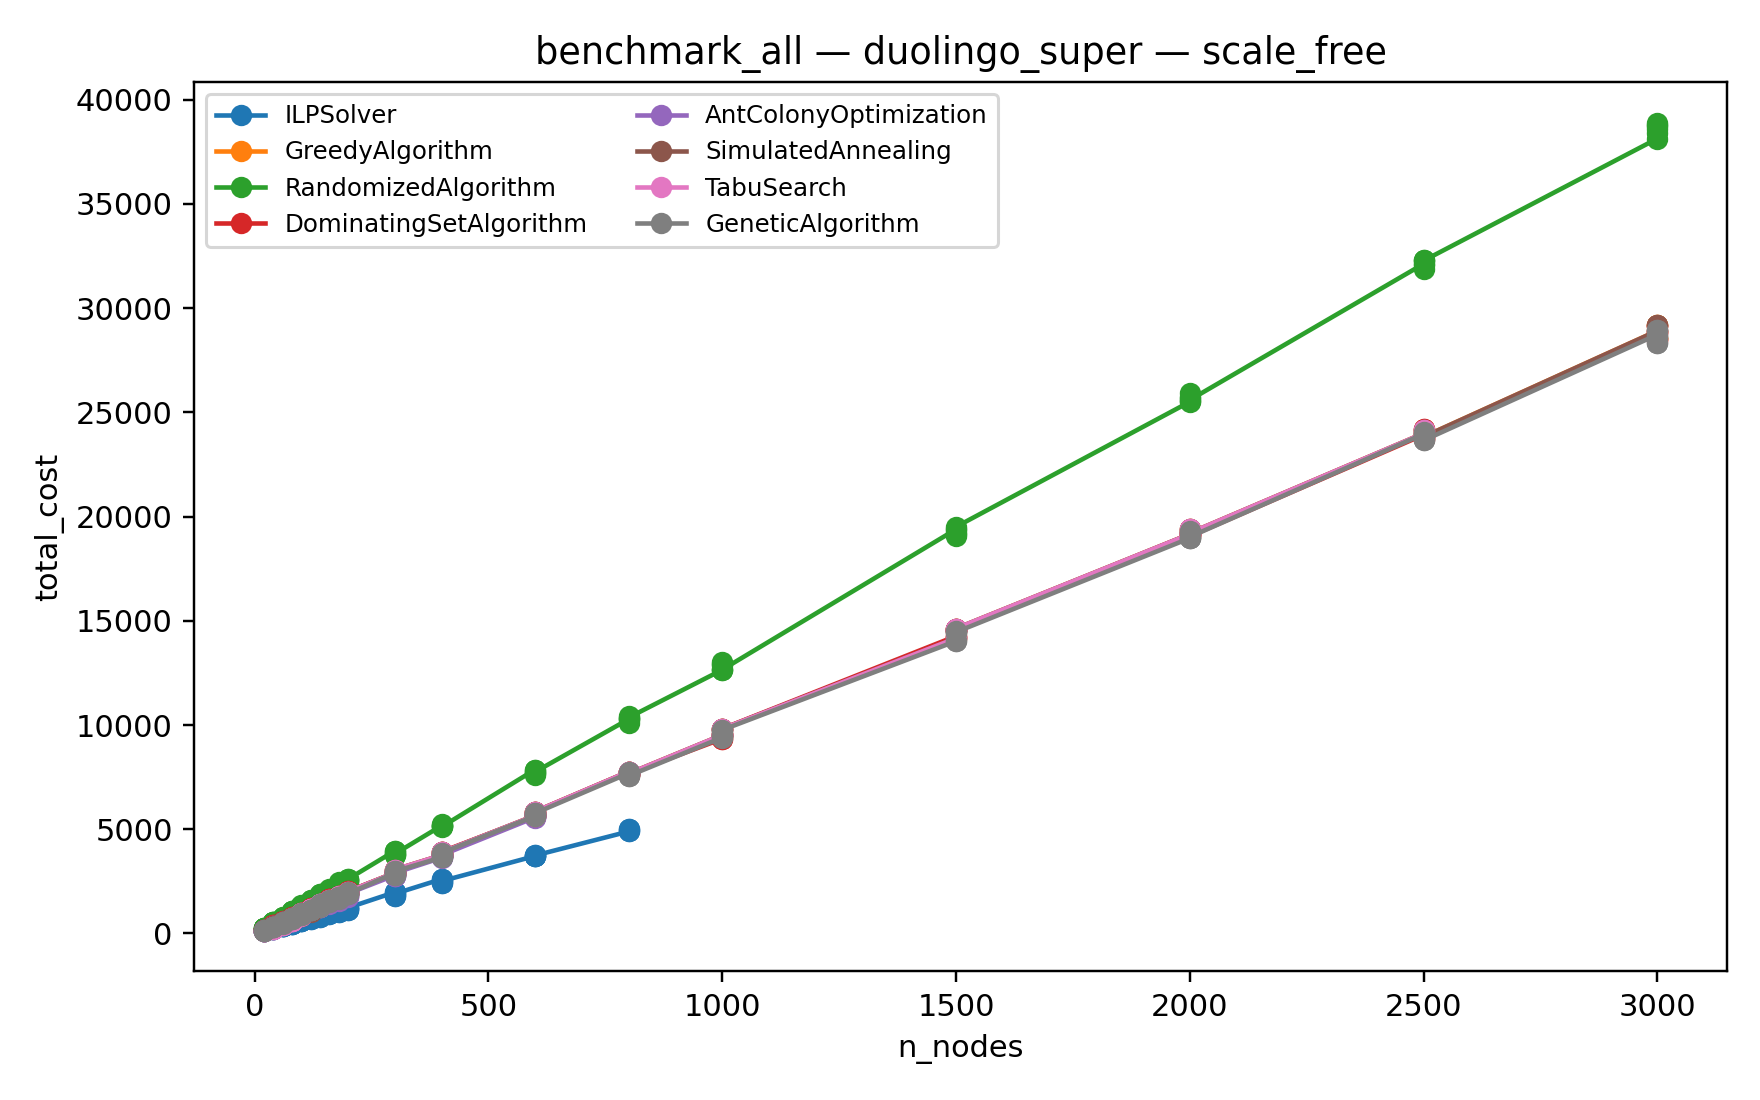
\includegraphics[width=0.48\linewidth]{assets/figures/ba_scale_free_duo_cost_vs_n.png}
  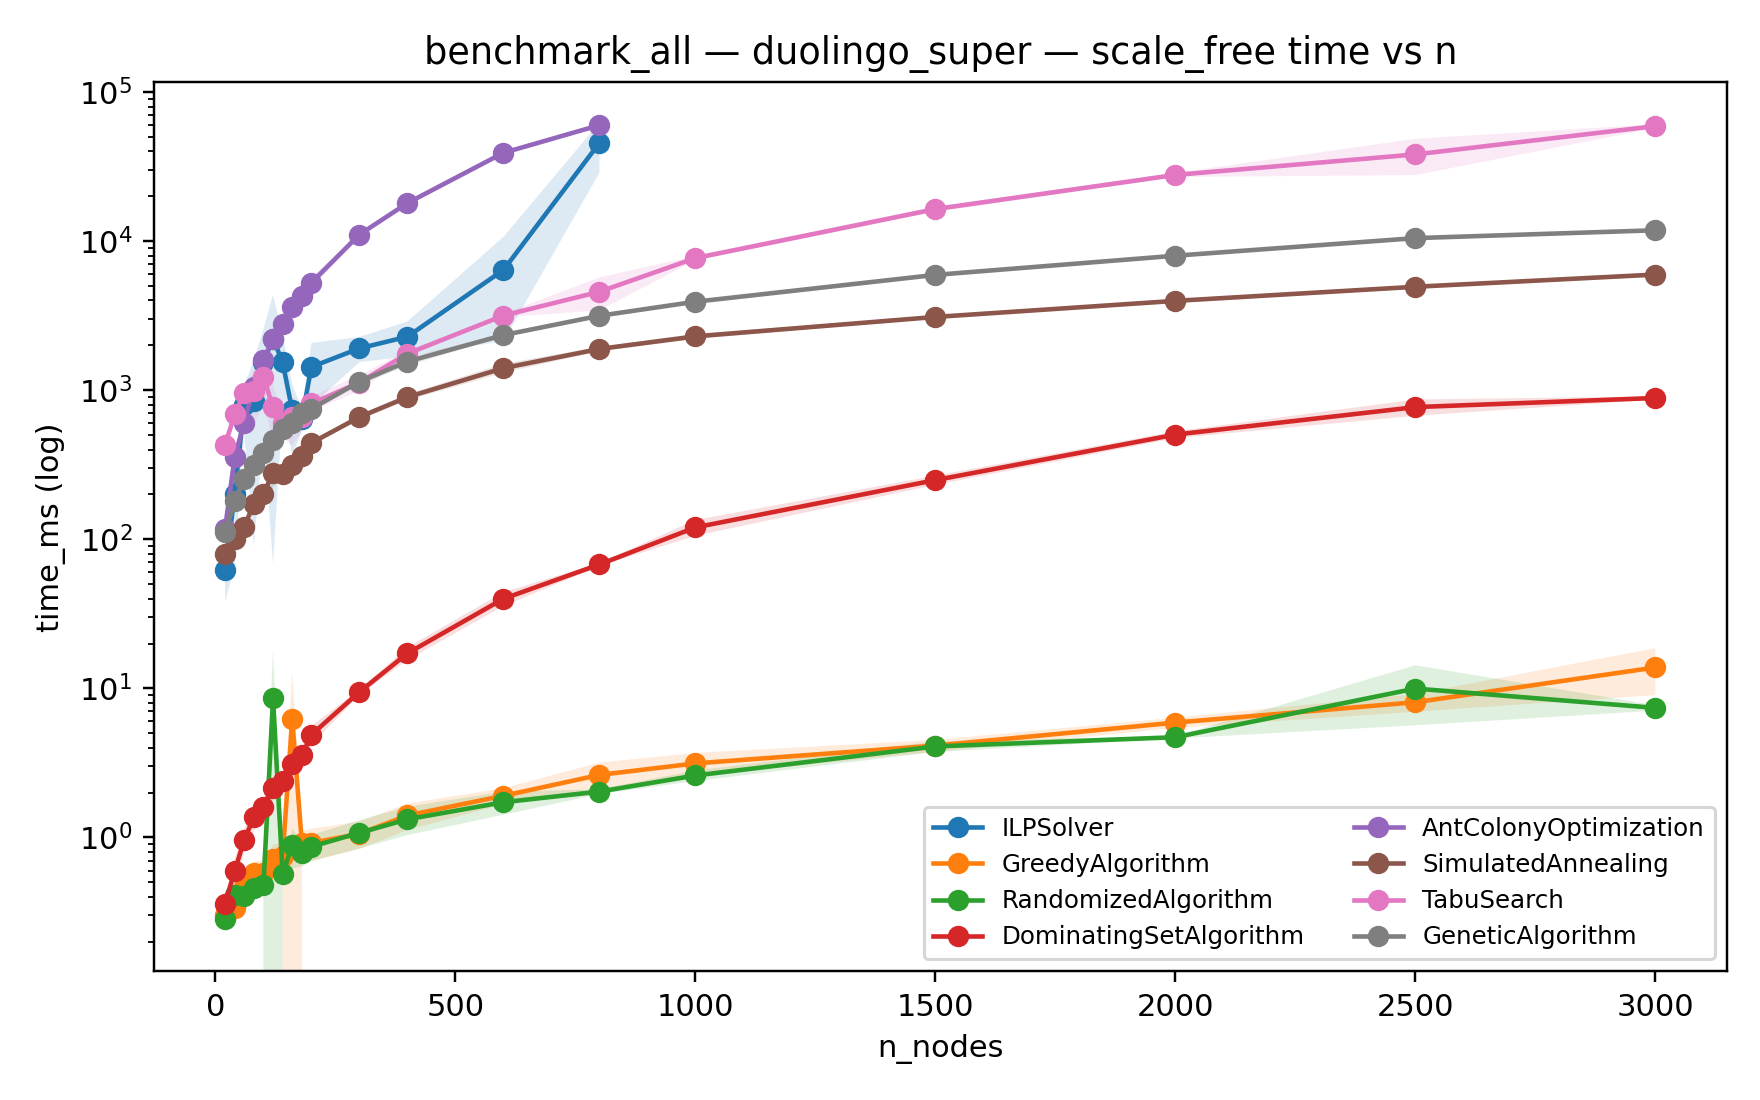
\includegraphics[width=0.48\linewidth]{assets/figures/ba_scale_free_duo_time_vs_n.png}
  \caption{Grafy bezskalowe (konf. duolingo\_super) -- koszt na wierzchołek i czas wykonania vs liczba wierzchołków.}
  \label{fig:scale_free_performance}
\end{figure}

\begin{figure}[H]
  \centering
  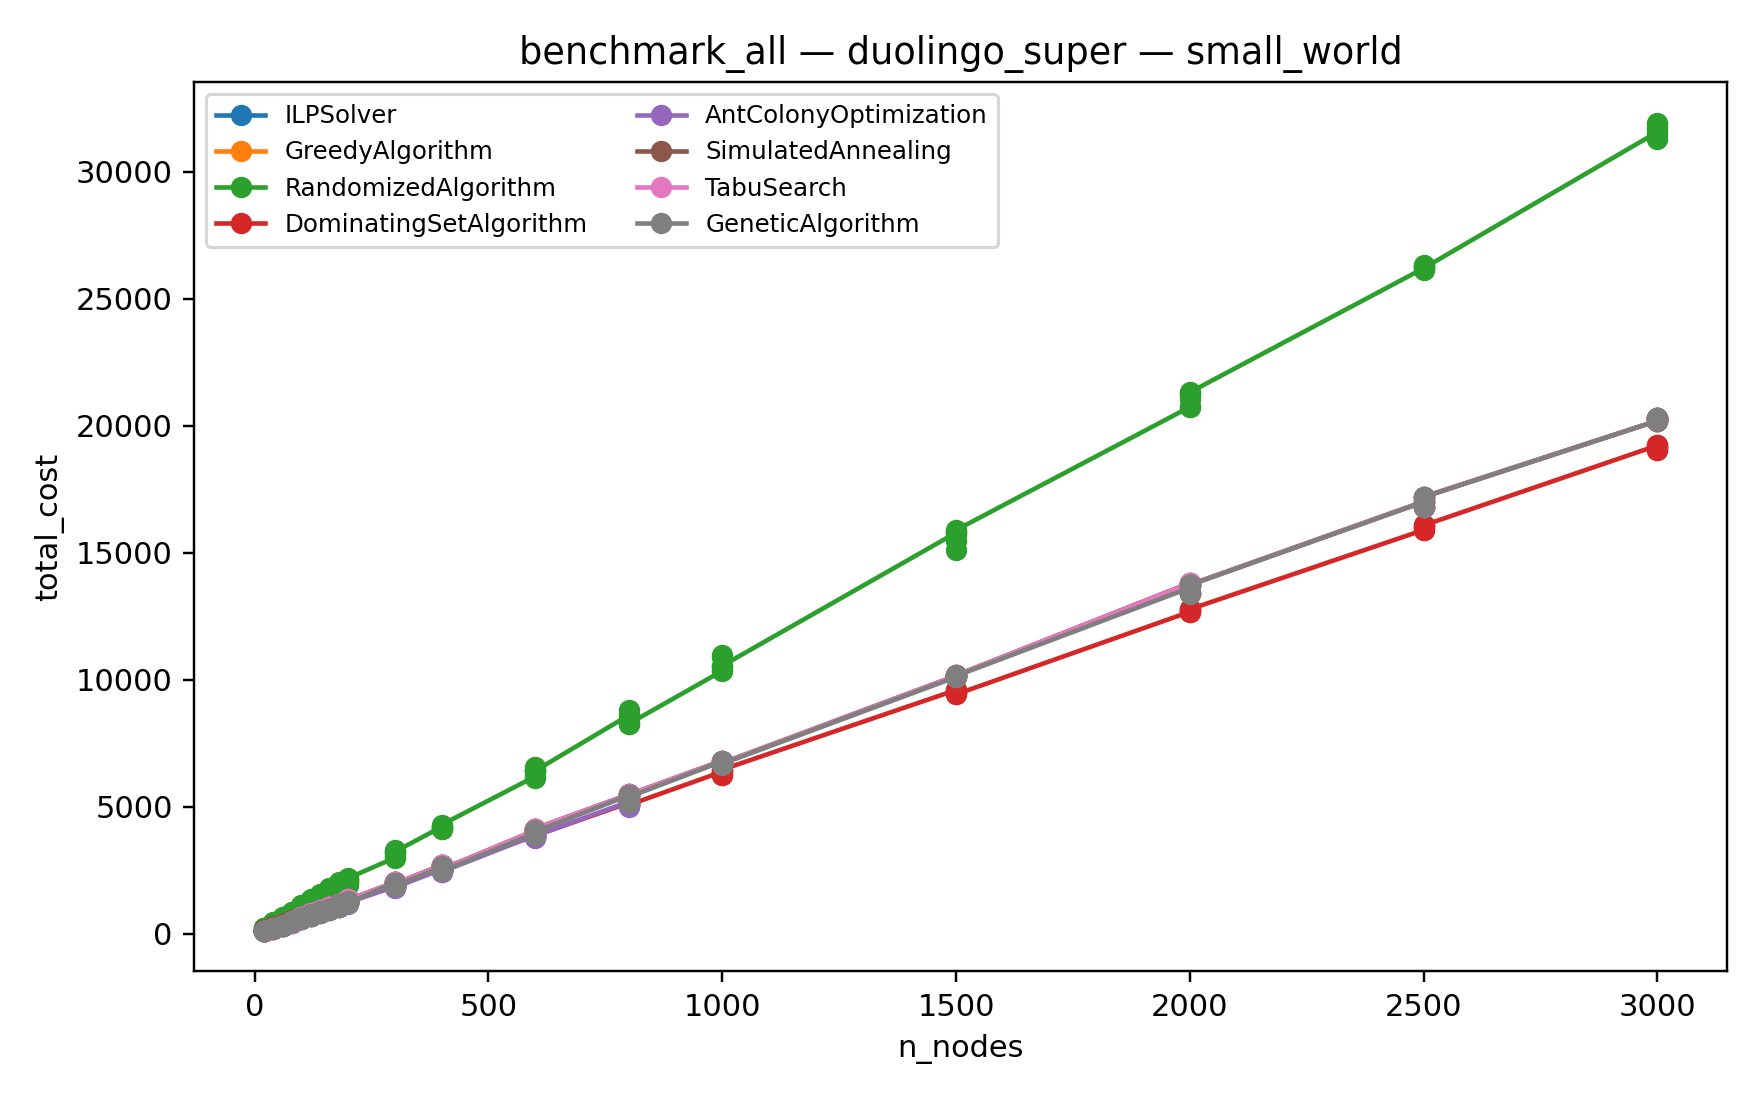
\includegraphics[width=0.48\linewidth]{assets/figures/ba_small_world_duo_cost_vs_n.png}
  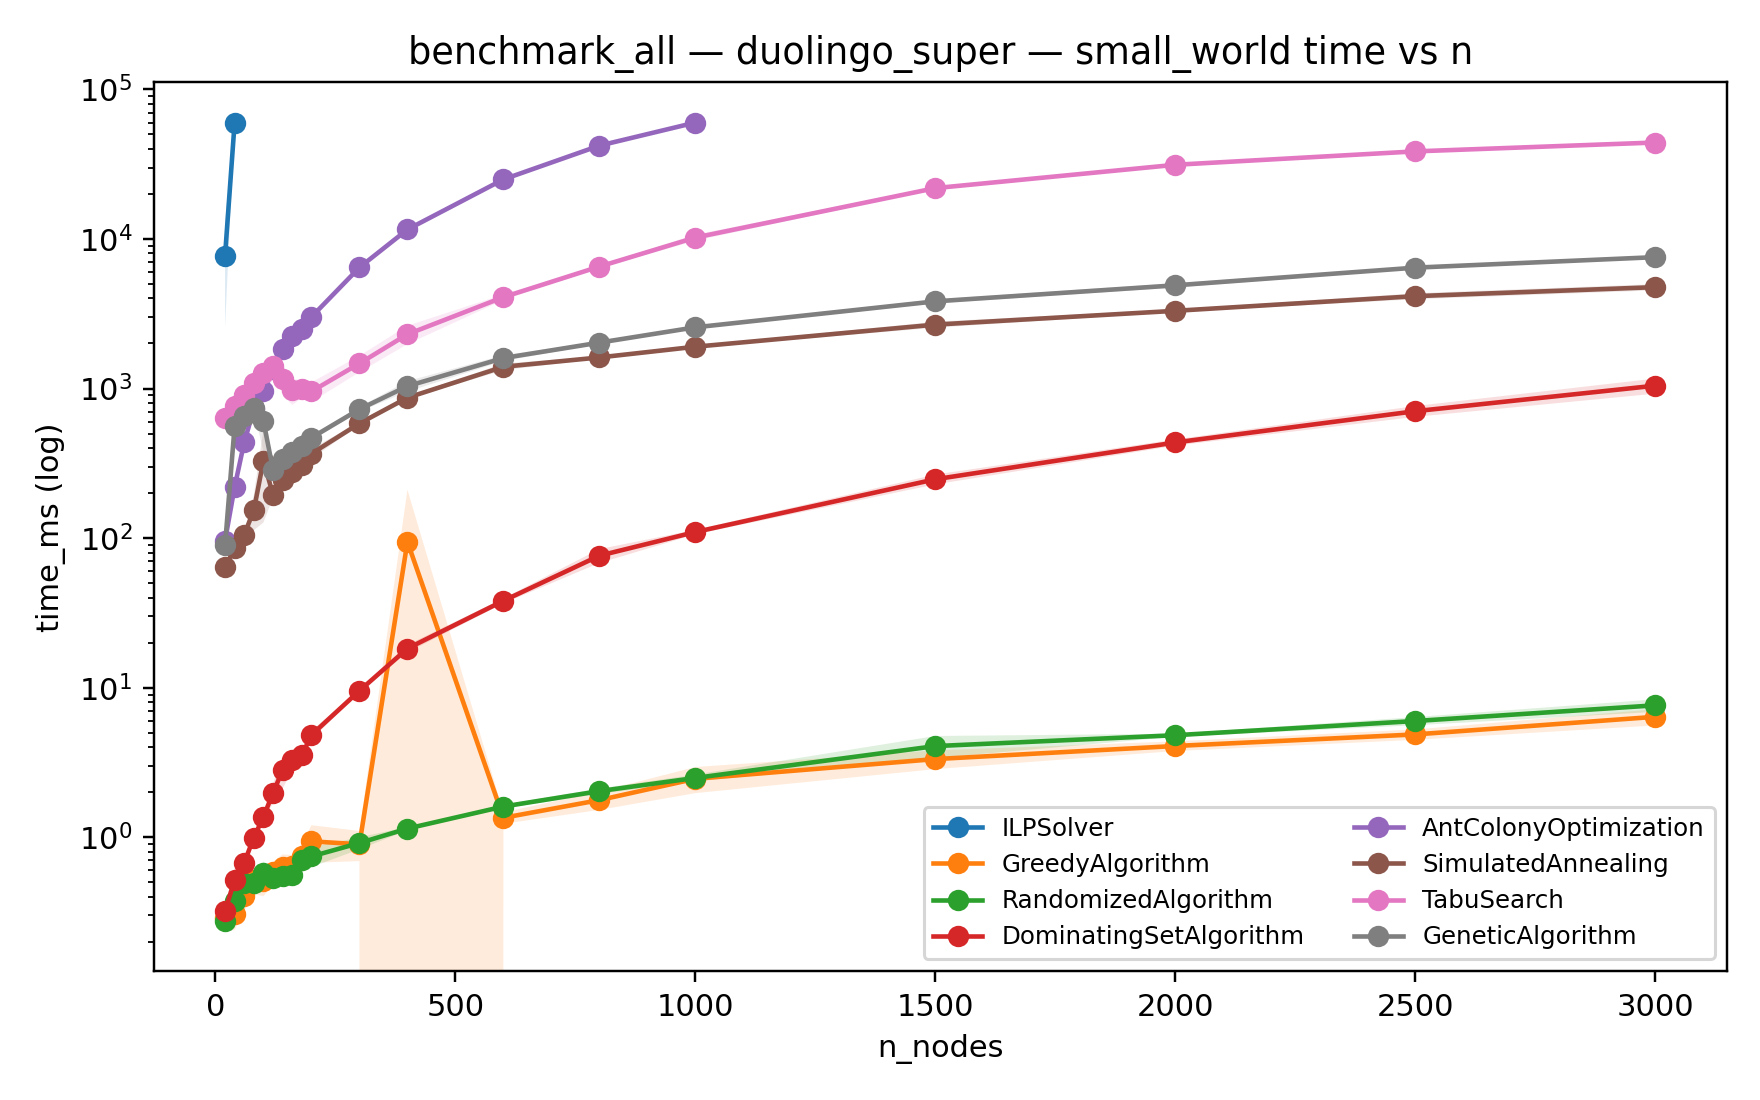
\includegraphics[width=0.48\linewidth]{assets/figures/ba_small_world_duo_time_vs_n.png}
  \caption{Grafy małoświatowe (konf. duolingo\_super) -- koszt na wierzchołek i czas wykonania vs liczba wierzchołków.}
  \label{fig:small_world_performance}
\end{figure}

Z wykresów wynika kilka ważnych obserwacji:

\paragraph{Jakość rozwiązań}
Metaheurystyki (algorytm genetyczny, symulowane wyżarzanie, tabu search, ant colony) dają najniższe koszty, ale są znacznie wolniejsze. Algorytm zachłanny (greedy) oferuje dobry kompromis -- jest szybki i daje wyniki tylko nieznacznie gorsze niż metaheurystyki.

\paragraph{Czas wykonania}
ILP bardzo szybko staje się niepraktyczny -- już dla grafów powyżej 100-200 wierzchołków przekracza limit czasu 60 sekund. Heurystyki konstrukcyjne (greedy, random, dominating set) są bardzo szybkie nawet dla dużych grafów.

\paragraph{Wpływ struktury grafu}
Grafy bezskalowe pozwalają na niższe koszty niż losowe czy małoświatowe — huby umożliwiają tworzenie większych, bardziej efektywnych grup licencyjnych (por. Rys.\,\ref{fig:scale_free_performance}). W grafach małoświatowych wysoki clustering sprzyja tworzeniu grup lokalnych, ale silne nakładanie się sąsiedztw ogranicza \emph{unikalne} pokrycie na krok, co tłumaczy przewagę heurystyk, które maksymalizują \emph{pokrycie per koszt} (DS) nad prostą kolejnością po stopniu (Rys.\,\ref{fig:small_world_performance}).

\subsection{Komentarz interpretacyjny i porównanie metod}
\label{subsec:interpretation}
Poniżej syntetyzujemy wnioski z wykresów (Rys.\,\ref{fig:random_performance}–\ref{fig:small_world_performance}, \ref{fig:pareto_analysis}, \ref{fig:facebook_results}):
\begin{itemize}
  \item \textbf{Greedy vs DS.} Na grafach bezskalowych (BA) prosta kolejność po stopniu jest bardzo skuteczna (Greedy \approx DS), gdyż kilku hubów zapewnia duże grupy rodzinne o niskim koszcie per osoba. W sieciach małoświatowych (WS) i losowych (ER) DS z kryterium \(\mathrm{coverage}/\mathrm{cost}\) częściej wybiera węzły o dobrym \emph{unikalnym} zasięgu, co obniża koszt bardziej niż Greedy.
  \item \textbf{Metaheurystyki.} GA/SA/TS/ACO zwykle poprawiają koszt względem Greedy/DS, szczególnie przy ograniczonych pojemnościach i mieszanej ofercie licencji, kosztem dłuższego czasu (fronty Pareto wskazują wyraźny kompromis między kosztem a czasem).
  \item \textbf{ILP.} Daje dolną granicę jakości na małych instancjach (walidacja heurystyk). Wraz ze wzrostem \(n\) i gęstości (Rys.\,\ref{fig:ilp_limits}) jego użyteczność spada — sensowne jest ustawianie limitu czasu i traktowanie wyniku jako górnej granicy dla metod przybliżonych.
  \item \textbf{Rzeczywiste sieci.} Na ego-sieciach Facebooka (Rys.\,\ref{fig:facebook_results}) Greedy pozostaje najszybszy i konkurencyjny jakościowo; metaheurystyki uzyskują dalsze, umiarkowane zyski kosztowe przy większych nakładach czasu.
\end{itemize}

\subsection{Analiza dodatkowych czynników wpływających na wydajność}

\paragraph{Porównanie konfiguracji licencji}
Bezpośrednie porównanie kosztów między Duolingo Super (ceny rzeczywiste) a wariantem roman domination (koszty względne) nie jest miarodajne — różne skale cenowe w naturalny sposób przekładają się na różne średnie koszty. W tym rozdziale koncentrujemy się więc na trendach w obrębie danej konfiguracji (wpływ struktury grafu i \(n\)), a porównania wariantów modelu przedstawiamy w rozdz.\,\ref{chap:extensions} (np. krzywe roman\_p\_x, analiza Spotify).

\paragraph{Wpływ gęstości i struktury grafów}
\begin{figure}[H]
  \centering
  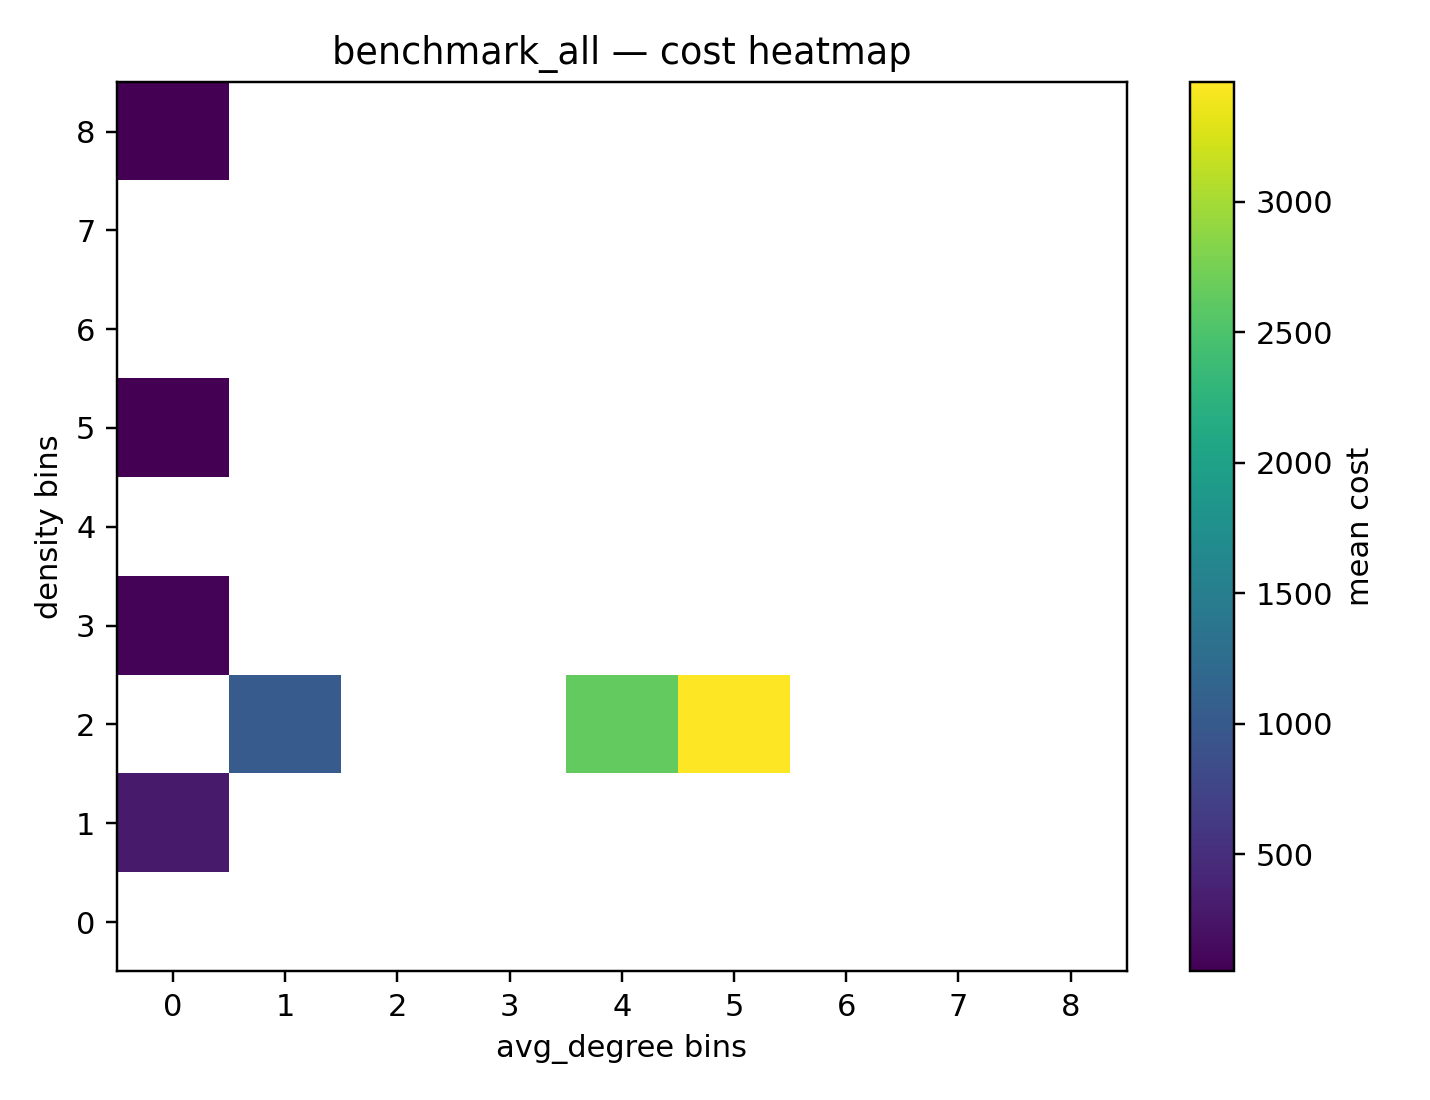
\includegraphics[width=0.7\linewidth]{assets/figures/ba_heatmap_cost.png}
  \caption{Heatmapa średniego kosztu na wierzchołek w zależności od gęstości i średniego stopnia grafu.}
  \label{fig:density_heatmap}
\end{figure}

Analiza wpływu topologii sieci na efektywność algorytmów ujawnia kluczową rolę gęstości grafu. Im więcej połączeń między węzłami, tym łatwiej algorytmom tworzyć duże grupy licencyjne, co przekłada się na obniżenie kosztu przypadającego na pojedynczy węzeł. Jednocześnie należy zauważyć, że gęstsze grafy wymagają proporcjonalnie więcej czasu na wykonanie obliczeń ze względu na zwiększoną złożoność kombinatoryczną problemu.

\paragraph{Analiza frontów Pareto}
Zastosowanie analizy Pareto pozwala na identyfikację rozwiązań niezdominowanych, gdzie żadne z rozwiązań nie jest jednocześnie tańsze i szybsze od pozostałych.

\begin{figure}[H]
  \centering
  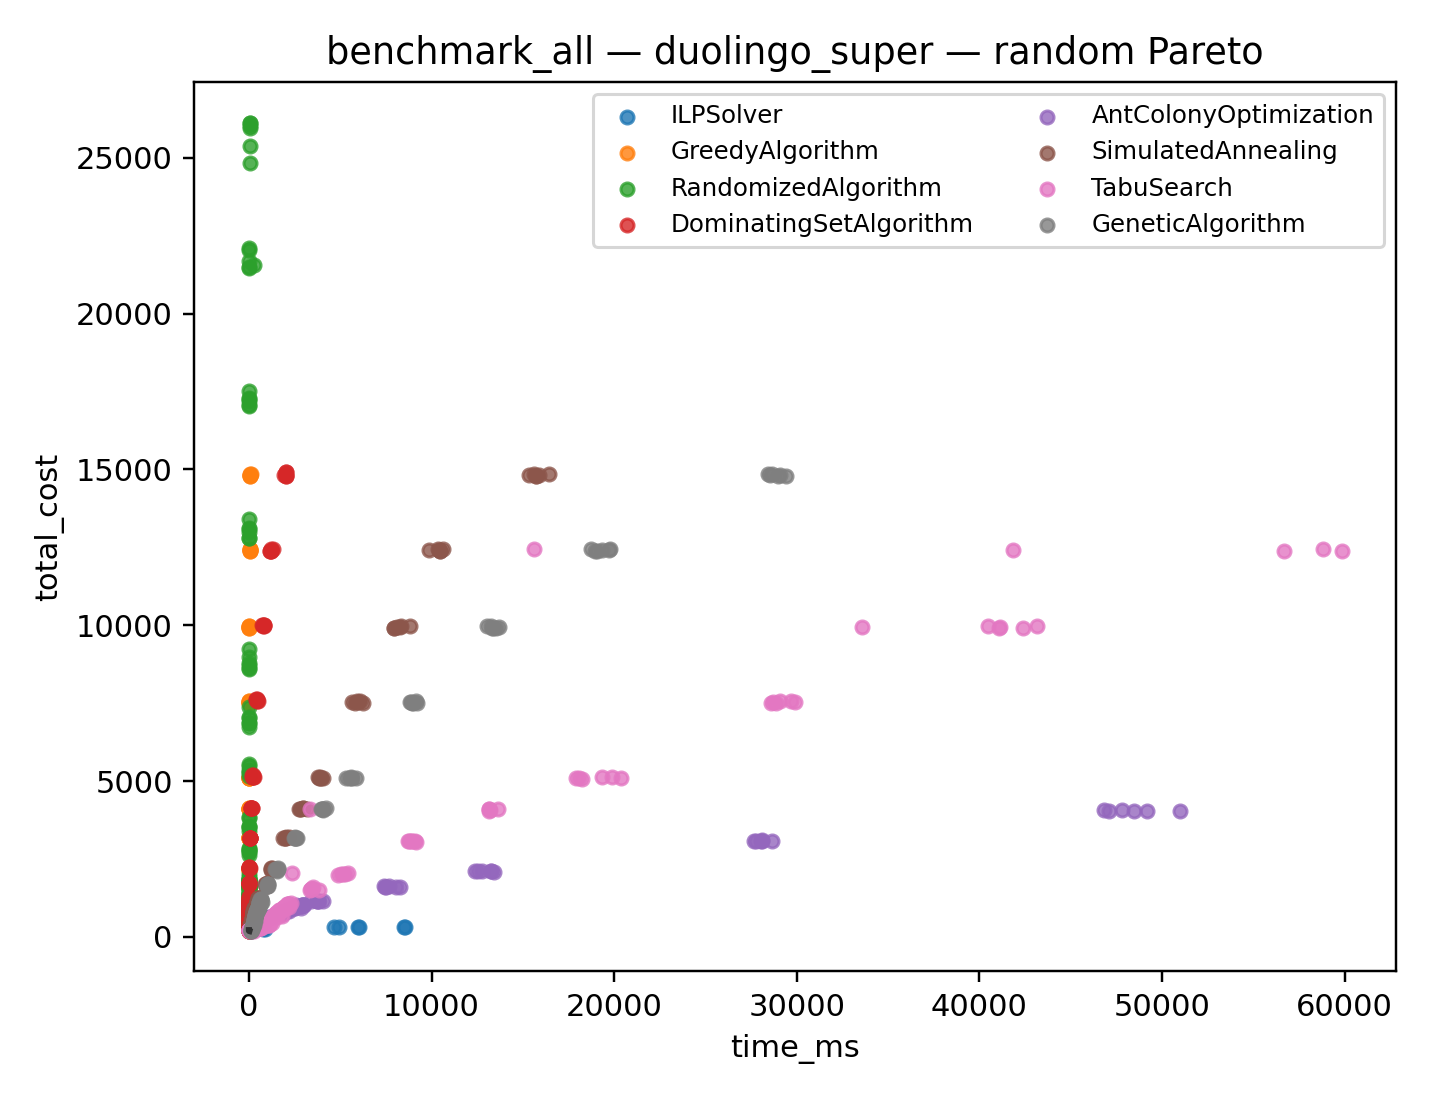
\includegraphics[width=0.48\linewidth]{assets/figures/ba_random_duo_pareto.png}
  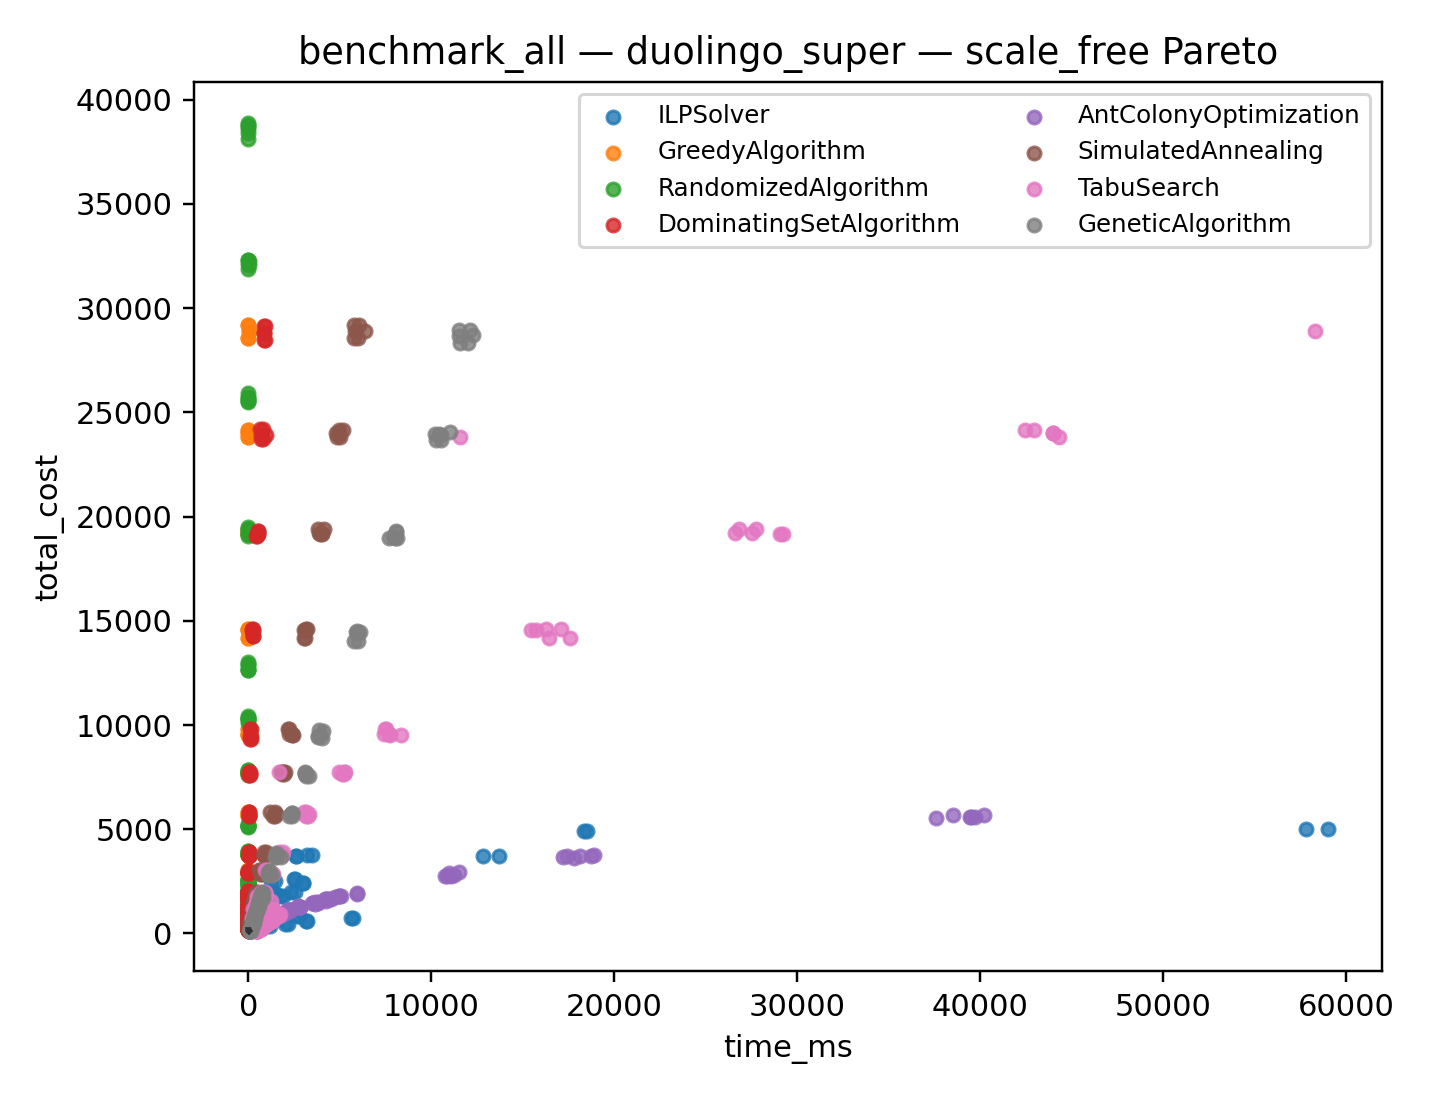
\includegraphics[width=0.48\linewidth]{assets/figures/ba_scale_free_duo_pareto.png}
  \caption{Fronty Pareto koszt vs czas dla grafów losowych (lewy) i bezskalowych (prawy), konf. duolingo\_super.}
  \label{fig:pareto_analysis}
\end{figure}

Na frontach Pareto widać:
\begin{itemize}
  \item Algorytm zachłanny oferuje najlepszy kompromis dla większości zastosowań
  \item ILP daje najniższy koszt, ale tylko dla małych grafów
  \item Metaheurystyki warto używać gdy czas nie jest krytyczny, a zależy nam na jak najniższym koszcie
\end{itemize}

\section{Wyniki uzupełniające i ograniczenia implementacyjne}

\subsection{Weryfikacja na grafach rzeczywistych}

\begin{figure}[H]
  \centering
  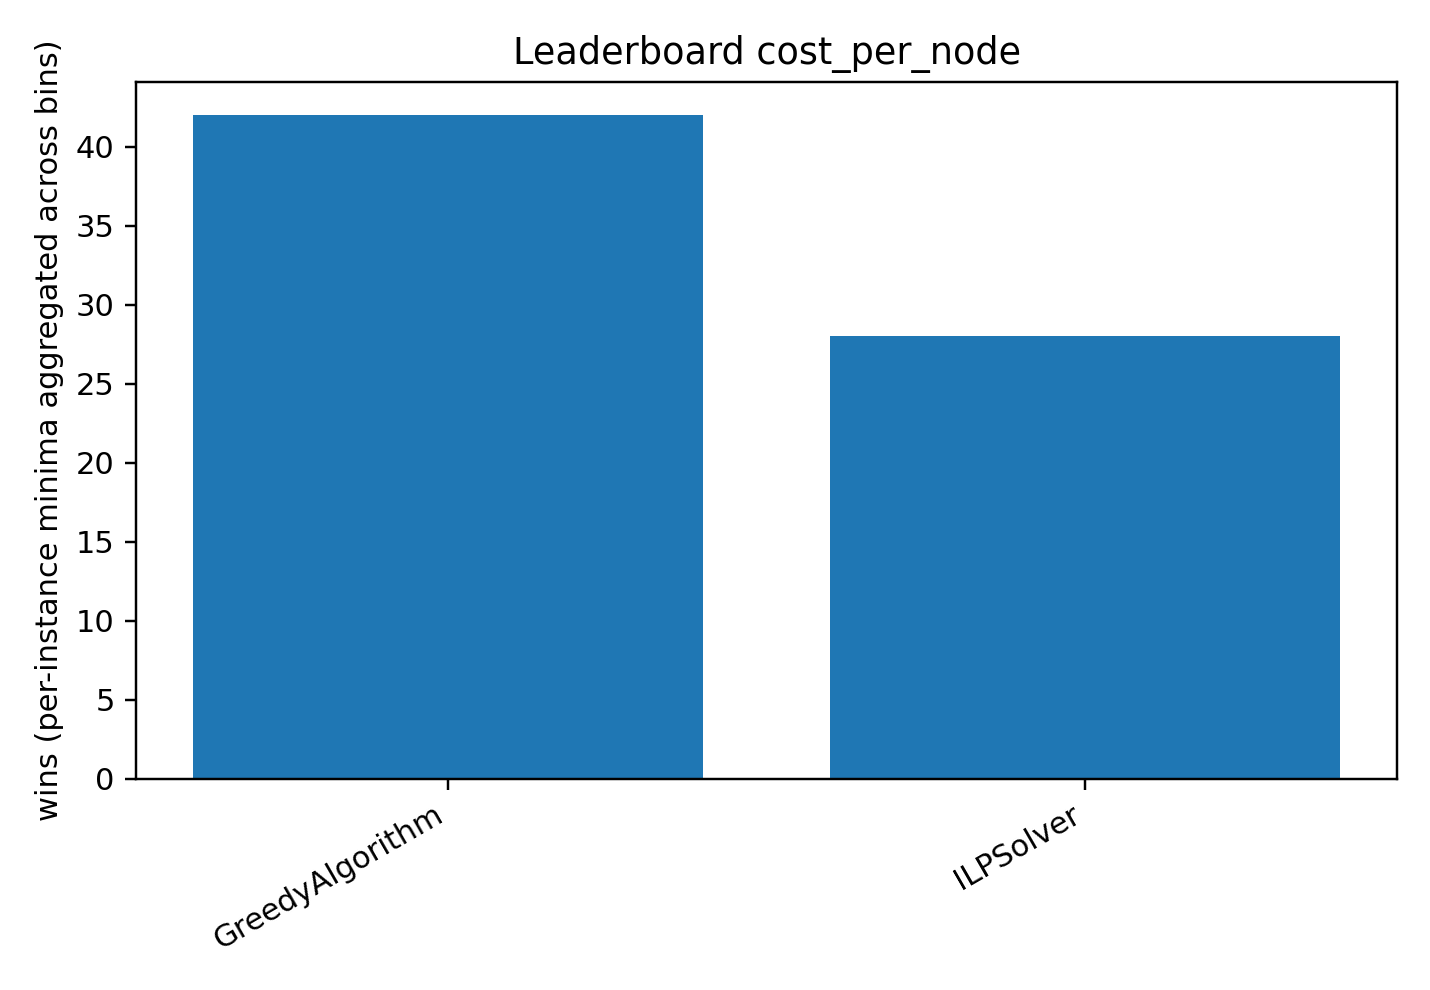
\includegraphics[width=0.48\linewidth]{assets/figures/br_leaderboard_cost.png}
  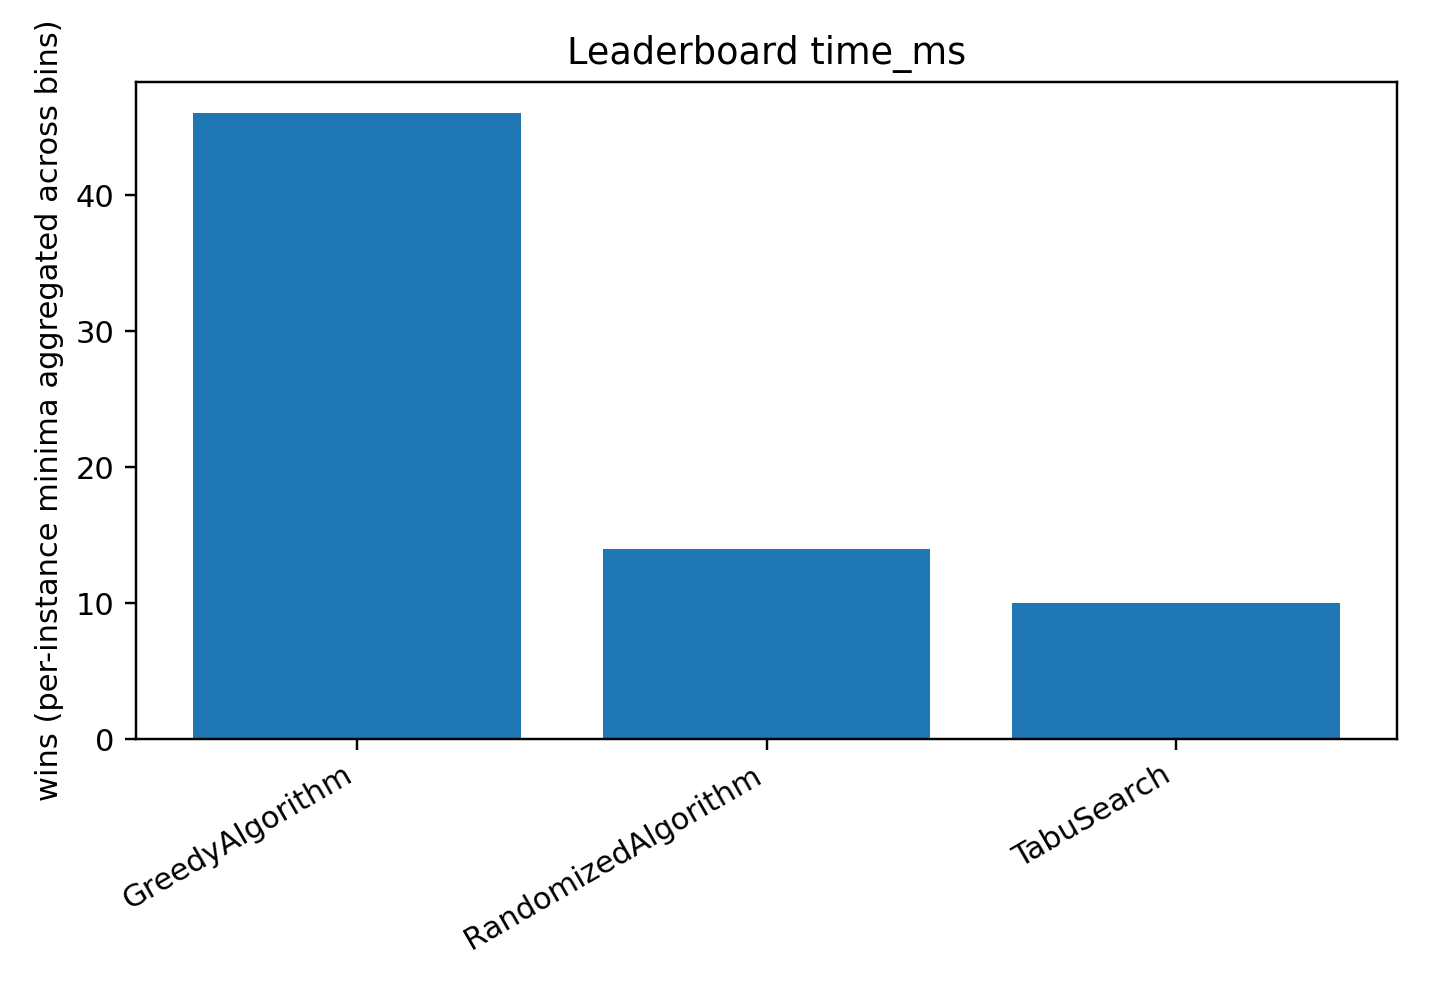
\includegraphics[width=0.48\linewidth]{assets/figures/br_leaderboard_time.png}
  \caption{Porównanie algorytmów na sieciach rzeczywistych (Facebook ego): koszt i czas.}
  \label{fig:facebook_results}
\end{figure}

Testowanie algorytmów na rzeczywistych sieciach ego z Facebooka potwierdza obserwacje poczynione dla grafów syntetycznych, wykazując wysoką spójność wyników między różnymi typami struktur sieciowych. Algorytm zachłanny konsekwentnie oferuje najkorzystniejszy kompromis między szybkością działania a jakością rozwiązań, podczas gdy metaheurystyki zapewniają umiarkowaną poprawę kosztów przy akceptacji znacznie dłuższych czasów obliczeniowych.

\subsection{Analiza granic skalowalności programowania liniowego}

Zastosowanie metod programowania liniowego (ILP) dostarcza rozwiązań optymalnych, jednak podlega istotnym ograniczeniom czasowym, które determinują praktyczną stosowalność tej metody. Rysunek przedstawiający granice czasowe solvera CBC ilustruje progowy charakter tego ograniczenia.

\begin{figure}[H]
  \centering
  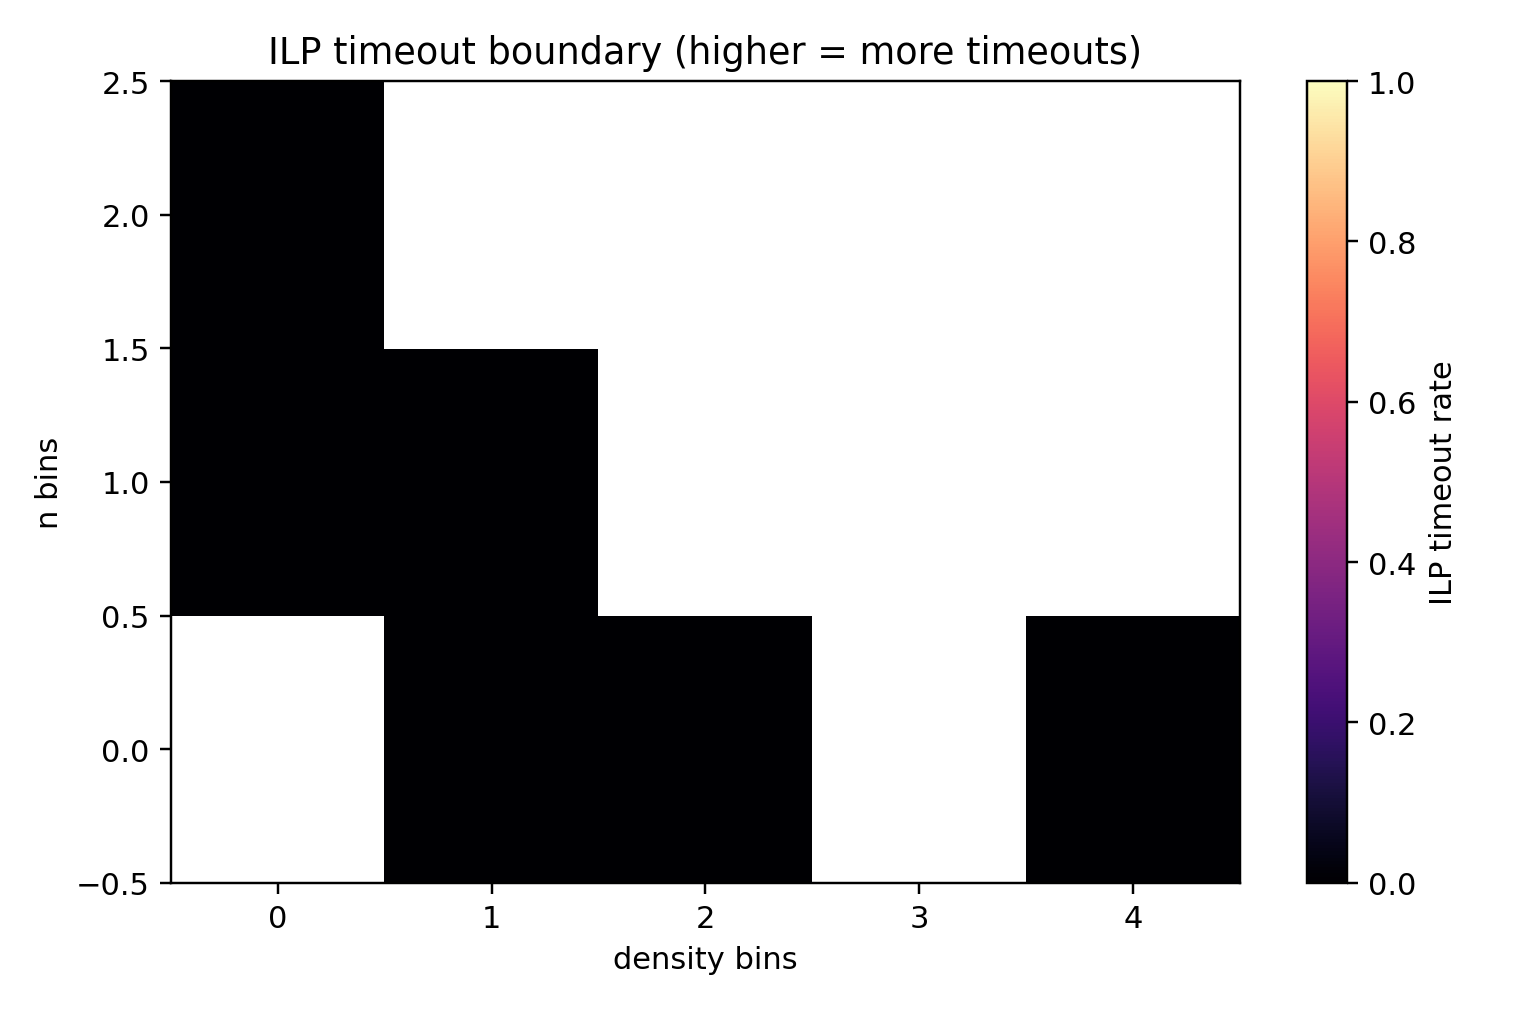
\includegraphics[width=0.7\linewidth]{assets/figures/ba_ilp_timeout_boundary.png}
  \caption{Granice czasowe ILP (solver CBC) w zależności od rozmiaru i gęstości grafu.}
  \label{fig:ilp_limits}
\end{figure}

Analiza wykazuje, że solver ILP zachowuje efektywność dla grafów zawierających do około 100-200 wierzchołków przy standardowej gęstości połączeń. Powyżej tej granicy krytycznej obserwuje się gwałtowny wzrost częstotliwości przekroczeń limitu czasowego, co czyni niezbędnym zastosowanie metod heurystycznych dla problemów większej skali.

\section{Końcowe wnioski}

\paragraph{Kluczowe obserwacje eksperymentalne:}
\begin{itemize}
  \item \textbf{Algorytm zachłanny} stanowi optymalny wybór dla większości zastosowań praktycznych, łącząc wysoką szybkość działania z satysfakcjonującą jakością rozwiązań
  \item \textbf{Programowanie liniowe (ILP)} zapewnia rozwiązania optymalne, lecz jego stosowalność ogranicza się do grafów małych rozmiarów (do około 100-200 wierzchołków)
  \item \textbf{Algorytmy metaheurystyczne} rekomenduje się w sytuacjach, gdy czas wykonania nie stanowi ograniczenia krytycznego, a priorytetem jest minimalizacja kosztów
  \item \textbf{Topologia grafu} wywiera decydujący wpływ na efektywność -- obecność węzłów o wysokim stopniu oraz zwiększona gęstość połączeń sprzyjają redukcji kosztów
\end{itemize}

\paragraph{Zalecenia dla implementacji praktycznych:}
W kontekście systemu dystrybucji licencji w sieciach społecznościowych zaleca się implementację algorytmu zachłannego jako domyślnej metody optymalizacji, z możliwością dynamicznego przełączania na algorytmy metaheurystyczne w przypadkach, gdy dla klientów o szczególnym znaczeniu każda minimalizacja kosztów ma istotną wartość biznesową.

\paragraph{Strategia doboru algorytmu:}
Analiza frontów Pareto jednoznacznie potwierdza brak uniwersalnego algorytmu optymalnego dla wszystkich scenariuszy -- wybór metody powinien być uwarunkowany priorytetami aplikacyjnymi:
\begin{itemize}
  \item W przypadku krytycznych ograniczeń czasowych -- zastosowanie algorytmu zachłannego
  \item Przy priorytetyzacji minimalizacji kosztów -- wykorzystanie metod metaheurystycznych
  \item Dla sieci małych rozmiarów ($<200$ węzłów) -- implementacja rozwiązania opartego na programowaniu liniowym
  \item W kontekście sieci rozległych -- metaheurystyki z inicjalizacją warm start algorytmem zachłannym
\end{itemize}
